\documentclass[UTF8,a4paper,12pt]{ctexart}

\usepackage{amsmath,amssymb,bm}
\usepackage{amsthm}
\usepackage{graphicx}
\usepackage{subcaption}
\usepackage{geometry}
\usepackage{booktabs}
\usepackage{float}
\usepackage{hyperref}
\usepackage[backend=biber,style=gb7714-2015,sorting=none]{biblatex}

\addbibresource{refs/cited.bib}

\renewcommand*{\bibfont}{\small}
\DeclareSourcemap{
  \maps[datatype=bibtex]{
    \map{
      \step[fieldset=doi, null]
      \step[fieldset=url, null]
      \step[fieldset=urldate, null]
      \step[fieldset=eprint, null]
    }
  }
}

\geometry{left=2.6cm,right=2.6cm,top=2.6cm,bottom=2.6cm}
\hypersetup{colorlinks=true,linkcolor=blue,citecolor=blue,urlcolor=blue}
\setlength{\parindent}{2em}
\setlength{\emergencystretch}{1.5em}
\setlength{\parskip}{0.15em}
\setlength{\abovedisplayskip}{6pt plus 2pt minus 2pt}
\setlength{\belowdisplayskip}{6pt plus 2pt minus 2pt}

% --- Theorem environments ---
\theoremstyle{definition}
\newtheorem{assumption}{假设}[section]
\newtheorem{definition}{定义}[section]
\newtheorem{problem}{问题}[section]

\theoremstyle{plain}
\newtheorem{theorem}{定理}[section]
\newtheorem{lemma}{引理}[section]
\newtheorem{proposition}{命题}[section]
\newtheorem{corollary}{推论}[section]

\theoremstyle{remark}
\newtheorem{remark}{注}[section]

\newcommand{\sgn}{\operatorname{sgn}}
\newcommand{\sig}{\operatorname{sig}}
\newcommand{\dd}{\mathrm{d}}
\newcommand{\R}{\mathbb R}

\title{基于漏斗预设性能与光滑周期延迟反馈的\\自由漂浮空间机械臂预设时间轨迹跟踪控制}
\date{}

\begin{document}

\maketitle

\begin{abstract}
针对捕获前自由漂浮空间机械臂基座不受控、关节动力学强耦合且末端轨迹跟踪同时要求瞬态包络与可预设收敛时间的问题，本文提出一种“漏斗预设性能—周期延迟零化”两段式控制方法。其基本观察是：预设性能控制（PPC）只约束误差的\emph{路径}而不约束其\emph{时间}，光滑周期延迟反馈（PDF）只约束误差的\emph{时间}而不约束其\emph{路径}，二者语义正交；但 PPC 的时变非线性误差变换会破坏 PDF 单周期零化所依赖的线性周期时滞结构，故不能在全程叠加。为此，本文先利用动量守恒将浮基动力学约化为等效关节空间模型，再用计算力矩补偿把误差通道化为严格解耦的二阶积分器；随后在观测阶段嵌入漏斗型预设性能律，构造与观测器收敛节奏同构、在预设时刻\emph{精确到达}稳态半径的指定时间可达性能函数；观测器本身按\(T_o\) 一分为二：\(T_o\) 前用奇异增益的二阶动量观测器完成预设时刻收敛，\(T_o\) 后切换为超螺旋滑模观测器精确保持零误差；最后在切换时刻无缝激活 Gramian 型 PDF，由单周期零化完成精确归零。主要结论为：(i) 在阶段 I 残差有限时，漏斗型控制律保持严格包络；其进带深度依赖残差上界，但包络结构不需要预先知道该上界；(ii) 在扰动变化率有限且超螺旋增益满足标准条件的条件下，阶段 II 通道无扰动，精确 Gramian PDF 对任意有界交接状态在 \(T_o+2h\) 归零；(iii) 全程包络还需严格的阶段 II 离线判据，且要求交接状态满足符号条件；本文据此给出可离线校验的三步参数规则，使 PDF 阶段的误差单调收敛；(iv) 观测残差、Gramian 数值误差与离散实现下，在周期递推条件成立且收缩因子小于 1 时给出含初态项的有限时间界和最终有界性。在七自由度浮基机械臂（文献 259 参数、\(20\,\mathrm{N\cdot m}\) 限幅、预设总时间 \(7\,\mathrm{s}\)）上的数值实验表明：预设性能阶段的包络违反时长为 \(0.178\,\mathrm{s\cdot joint}\)（占该阶段关节—时间总长的 \(0.5\%\)，归一化比峰值 \(1.11\)），而同一包络下纯基准反馈违反 \(9.8\,\mathrm{s\cdot joint}\)、归一化比峰值 \(12.0\)；进带深度为误差带的 \(2.1\%\!-\!90.7\%\)。针对 PPC 不约束交接速度所造成的 PDF 阶段位置外扩，本文给出“交接符号条件—末段速度阻尼—自由/注入窗口校验”的三步参数规则：按该规则（\(T_o=5\,\mathrm{s}\) 时 \(\delta=0.4\,\mathrm{s}\)、\(k_v=20\)）把交接速度由 \(3.2\times10^{-2}\) 压到 \(2.5\times10^{-4}\,\mathrm{rad/s}\) 后，PDF 阶段的误差范数单调、各关节无超调（最大越界比由 \(5.38\) 降至 \(0.907<1\)、包络违反时长为 0）；采样实现的稳态残差为 \(4.6\times10^{-5}\,\mathrm{rad}\) 并随步长线性下降（\(T_s\) 减半至 \(2.3\times10^{-5}\)），与命题 4.2 的最终有界结论一致。
\end{abstract}

\noindent\textbf{关键词：}自由漂浮空间机械臂；预设性能控制；预设时间控制；周期延迟反馈；单周期零化；扰动观测器

\section{引言}
\label{sec:intro}

空间机械臂是执行在轨服务、碎片清理与失效航天器维护的核心装备~\cite{liu2021review,yan}。捕获前的机械臂通常处于自由漂浮状态：基座不施加主动控制，关节运动通过动量守恒诱导基座反作用运动，使末端轨迹偏离固定基座假设下的标称值。因此，在基座不受控、动力学强耦合的条件下同时保证\emph{瞬态行为可设计}与\emph{收敛时间可预设}，是自由漂浮空间机械臂控制的关键问题。

\paragraph{建模与跟踪控制}
Umetani 与 Yoshida 的广义雅可比矩阵奠定了速度级建模基础~\cite{umetani1989}；Vafa 与 Dubowsky 的虚拟机械臂方法从动量守恒刻画了运动学—动力学耦合~\cite{vafa1990}；Papadopoulos 与 Dubowsky 揭示了动力学耦合引起的动态奇异~\cite{papadopoulos1993,dubowsky1993}。控制层面，已有自适应计算力矩~\cite{parlaktuna2004}、零反作用控制~\cite{xu2016}、约束轨迹优化~\cite{wang2015}、模型预测跟踪~\cite{ning2019}与滑模/时延估计复合方案~\cite{yu2022}。这些方法在精度与鲁棒性上各有侧重，但收敛时间通常依赖增益与初始状态的复杂关系，难以在设计阶段独立指定。

\paragraph{预设性能控制}
预设性能控制（PPC）通过性能函数与误差变换定量刻画收敛速度、超调与稳态精度 ~\cite{katsoukisLowComplexityRobust2022}。空间机器人领域已有障碍李雅普诺夫与神经网络复合的预设性能方案 ~\cite{yao2021}、预设性能与约束固定时间终端滑模的结合 ~\cite{huConstrainedFixedTimeTerminal2024}、执行器故障下的柔性预设性能策略 ~\cite{liErrorTriggeredFlexiblePrescribed2025}，以及预设性能与观测器的融合设计 ~\cite{chenPrescribedPerformanceObservercontroller2025}。其共同优点是瞬态可定量设计，但性能函数多具无限时间到达特性或依赖精确初始误差，\emph{收敛时间上界本身不是设计参数}。

\paragraph{预设时间控制}
固定/预定义/指定时间控制可给出与初始状态无关的收敛上界：Polyakov 基于非连续齐次性建立了固定时间框架~\cite{polyakov2012}，Zuo 等推广至一致性~\cite{zuo2019}，Su 等实现机械臂固定时间跟踪~\cite{su2020}；相关研究将预定义时间思想用于 SE(3) 位姿跟踪~\cite{xuPredefinedTimeTrackingControl2024}，将分数阶非奇异终端滑模用于自由漂浮机械臂~\cite{dou2025fractional}，以及含执行器故障与性能约束的固定时间容错控制~\cite{li2025}。此类方法多依赖非光滑滑模面或分数幂反馈，在收敛时刻附近存在控制跳变与增益奇异。

\paragraph{光滑周期延迟反馈}
Pyragas 的延迟反馈通过“当前状态与延迟一个周期状态之差”镇定不稳定周期轨道~\cite{pyragas1992}。Zhou 等将其延拓为光滑周期延迟反馈（PDF）：对可控线性时滞系统，通过设计 \(2h\) 周期增益使单周期状态转移矩阵零化，在 \(2h\) 后\emph{精确}归零，且增益可取得光滑从而避免终端奇异~\cite{zhouFixedtimeStabilizationLinear2022}；Ding 等进一步给出强预设时间镇定与不确定非线性推广~\cite{dingStrongPrescribedtimeStabilization2024}。PDF 的代价是要求对象已处于线性可控形式，且\emph{不提供到达前的任何瞬态刻画}。

\subsection{问题与本文思路}
\label{sec:intro_problem}

上两条路线存在天然的互补：PPC 约束\emph{路径}而不约束\emph{时间}，PDF 约束\emph{时间}而不约束\emph{路径}。但其直接叠加存在两处结构性障碍，这正是本文的出发点：

\begin{enumerate}
  \item[(a)] \textbf{变换破坏结构。}单周期零化 \(\Delta_K(h)=0\) 是线性周期时滞系统的代数性质，由可控 Gramian 反解得到。PPC 的时变非线性变换 \(e_i=\rho_i(t)S(\varepsilon_i)\) 会使闭环变为非线性泛函微分方程，\(\Delta_K(h)\) 失去定义；若对延迟状态也用同一性能函数，还会引入 \(\rho(t)\) 与 \(\rho(t-h)\) 不匹配的强迫项。
  \item[(b)] \textbf{峰值落在关键窗口。}预设时间扰动观测器（PTDO）收敛前存在观测峰值~\cite{jiangPrescribedtimeDisturbanceObserver2024}，而该峰值恰出现在 PPC 需要保包络的时段；若把观测残差简单当作扰动处理，则需要其先验上界，与“上界未必已知”的实际情形矛盾。
\end{enumerate}

本文的处理是让两种机制在\emph{时间上分段}而非在\emph{结构上叠加}，并把交接点取在观测器的预设收敛时刻 \(T_o\)：利用计算力矩补偿把误差通道化为严格解耦的二阶积分器，使漏斗设计退化为逐关节标量问题（无需反步、逼近与加速度测量）；构造与预设时刻观测器收敛节奏同构的指定时间可达性能函数，使其在 \(T_o\) 处精确到达稳态半径且二阶连续可微，与 PDF 激活时刻精确对齐；并证明漏斗界只要求残差\emph{有限}而与其数值\emph{无关}，从而观测峰值不破坏包络、只消耗“贴合深度”。

\subsection{主要贡献}
\begin{enumerate}
  \item 提出“漏斗预设性能—周期延迟零化”两段式结构（第~\ref{sec:controller}~节），给出总预设时间 \(T_{\mathrm{pre}}=T_o+2h\) 的双重预设结论：预设时间 \(T_o\) 内进入预设误差带，再经预设时间 \(2h\) 精确归零（定理~\ref{thm:main}）。
  \item 设计分段观测器（定理~\ref{thm:obs1}、\ref{thm:sta}）：\(T_o\) 之前用奇异增益的二阶动量观测器，在有限变化率条件下使 \(\hat d\to d(T_o)\) 且收敛界与初值无关；\(T_o\) 之后切换为超螺旋滑模观测器，在扰动导数有界的标准增益条件下\emph{保持}零误差，取代了旧版需要额外 Lyapunov 证书的单一预设时间观测器。
  \item 给出包络保持定理（定理~\ref{thm:ppc}）：\(\vartheta_i<1\) 对任意\emph{有限}观测残差成立，与残差幅度无关。据此证明 PPC 把观测峰值从“破坏精度”降级为“消耗进带余量”，并与纯 PD 的输入—状态界定量对照（推论~\ref{cor:pd_compare}）。
  \item 给出阶段 II 的包络校验判据 \(M_hB_o\le\min_i\rho_{i\infty}\)（命题~\ref{prop:stage2}），指出这是“预设包络”与“预设时间”\emph{不能同时无条件成立}的唯一结构瓶颈，它把人工延迟、Gramian 增益规模与误差带宽度显式耦合。
  \item 划出不可行边界（第~\ref{sec:infeasible}~节）：无观测器时归零不成立；超螺旋增益下界与采样/限幅上界之间存在定量三角约束；离散实现下结论退化为显式有界跟踪。
\end{enumerate}

\(\lVert\cdot\rVert\) 为 Euclidean 范数或诱导 2-范数，\(\lVert\cdot\rVert_\infty\) 为元素最大绝对值；\(\sgn(\cdot)\) 与 \(\sig^{\alpha}(x)=\sgn(x)\lvert x\rvert^{\alpha}\) 按元素作用，\(n\) 为关节数。

\section{动力学模型与问题描述}
\label{sec:model}

\subsection{等效关节空间模型}
\label{sec:modeling}

\begin{figure}
    \centering
    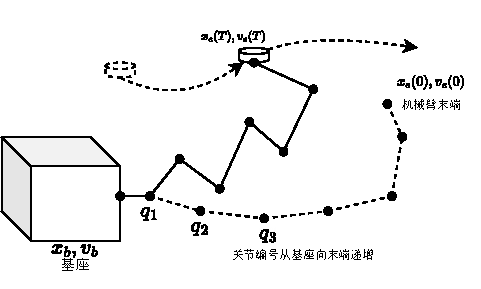
\includegraphics[width=0.8\textwidth]{assets/manipulator.drawio.pdf}
    \caption{空间抓取目标任务下的悬浮机械臂模型示意图}
    \label{fig:manipulator}
\end{figure}

% （此处 \(\dot x_b\) 仅记速度，不表示姿态坐标的普通导数）
如图\ref{fig:manipulator}所示，
设基座体坐标系中的广义速度 \(\dot x_b=[v_b^{\top},\omega_b^{\top}]^{\top}\in\R^{6}\)，关节变量 \(q = [q_1,q_2,\cdots, q_n]\in\R^{n}\)。
关节编号从基座向末端递增。
广义速度取体坐标系下的速度分量而非姿态坐标的导数；一般情形下惯性块可依赖基座姿态 \(g_b\) ，本文的自由漂浮设定下该依赖消失，故简记为  \(H(q)\)。
系统动能为二次型
\begin{equation}
T=\tfrac12\begin{bmatrix}\dot x_b^{\top}&\dot q^{\top}\end{bmatrix}
\begin{bmatrix}H_b&H_{bm}\\ H_{bm}^{\top}&H_m\end{bmatrix}
\begin{bmatrix}\dot x_b\\ \dot q\end{bmatrix},
\label{eq:kinetic}
\end{equation}
其中 \(H_b\in\R^{6\times6}\)、\(H_m\in\R^{n\times n}\)、\(H_{bm}\in\R^{6\times n}\)。由拉格朗日方程得完整动力学
\begin{equation}
\begin{bmatrix}H_b&H_{bm}\\ H_{bm}^{\top}&H_m\end{bmatrix}
\begin{bmatrix}\ddot x_b\\ \ddot q\end{bmatrix}
+\begin{bmatrix}C_b&C_{bm}\\ C_{bm}^{\top}&C_m\end{bmatrix}
\begin{bmatrix}\dot x_b\\ \dot q\end{bmatrix}
=\begin{bmatrix}0\\ \tau\end{bmatrix},
\label{eq:full_dynamics}
\end{equation}
第一行右端为零（基座不受控）；惯性块可由空间复合刚体算法以 \(O(n^{2})\) 复杂度计算。

设无外力矩且初始空间总动量为零；空间动量始终为零，经可逆的坐标变换后基座体坐标系动量也为零，故 \(H_b\dot x_b+H_{bm}\dot q=0\)，即
\begin{equation}
\dot x_b=-H_b^{-1}H_{bm}\dot q\triangleq J_{bm}(q)\dot q
\ \Longrightarrow\
\dot x_e=\bigl[J_m+J_bJ_{bm}\bigr]\dot q\triangleq J_g(q)\dot q ,
\label{eq:gjm}
\end{equation}
其前提是 \(H_b\) 在工作区域内一致正定。式~\eqref{eq:gjm}~表明基座运动是由关节运动诱导的反作用而非独立控制量。对 \(H_b\dot x_b+H_{bm}\dot q=0\) 求导并与 \eqref{eq:full_dynamics}~两行联立消去 \(\ddot x_b\)，得等效关节空间模型
\begin{equation}
M_e(g_b,q)\ddot q+c_e(g_b,q,\dot q)=\tau+d(t),\qquad
M_e(q)=H_m-H_{bm}^{\top}H_b^{-1}H_{bm},
\label{eq:ejm}
\end{equation}
其中 \(M_e\) 为 Schur 补，\(c_e\) 汇总递推动力学、动量约束求导与坐标变换产生的速度项，\(d(t)\) 为集总扰动。在选定坐标系下若 \(M_e\) 仅依赖关节、\(c_e=C_e(q,\dot q)\dot q\)，下文采用该简记；否则下列控制律中的 \(M_e,C_e\dot q\) 均须替换为完整的 \(M_e(g_b,q),c_e\)，并实时取得基座位姿以计算它们。将关节变量统一记为 \(q_m\)，后文使用的简记模型为
\begin{equation}
M_e(q_m)\ddot q_m+C_e(q_m,\dot q_m)\dot q_m=\tau+d(t).
\label{eq:model}
\end{equation}
式~\eqref{eq:model}~将原 \(6+n\) 维耦合系统降为 \(n\) 维。

\subsection{误差通道}
\label{sec:error_channel}

给定足够光滑的期望轨迹 \(q_d(t)\)，定义
\begin{equation}
e=q_m-q_d,\qquad \dot e=\dot q_m-\dot q_d,\qquad
z=\begin{bmatrix}e\\ \dot e\end{bmatrix}\in\R^{2n},
\label{eq:error_state}
\end{equation}
并取“计算力矩补偿 + 扰动补偿”结构
\begin{equation}
\tau=M_e(q_m)\bigl(\ddot q_d+\nu\bigr)+C_e(q_m,\dot q_m)\dot q_m-\hat d(t),
\label{eq:computed_torque}
\end{equation}
其中 \(\nu\in\R^{n}\) 为辅助加速度输入，\(\hat d\) 为扰动补偿量。


\subsection{性能函数与误差变换}
\label{sec:performance}

\begin{definition}[指定时间可达性能函数]\label{def:atpf}
称 \(\rho:\R_{\ge0}\to\R_{>0}\) 为可达时间 \(T_s\)、稳态半径 \(\rho_\infty\) 的指定时间可达性能函数，若 \textup{(i)} \(\rho\) 在 \([0,T_s)\) 上单调递减且为正；\textup{(ii)} \(\lim_{t\to T_s^-}\rho(t)=\rho_\infty>0\)；\textup{(iii)} \(\rho(t)\equiv\rho_\infty\) 于 \(t\ge T_s\)。
\end{definition}

\begin{definition}[误差变换函数]\label{def:transform}
称光滑严格递增的 \(S:\R\to(-1,1)\) 为误差变换函数，若 \(\lim_{\varepsilon\to\pm\infty}S(\varepsilon)=\pm1\)。对归一化误差 \(\xi_i=e_i/\rho_i\in(-1,1)\)，变换误差为 \(\varepsilon_i=S^{-1}(\xi_i)\)。
\end{definition}

对本文采用的 \(S=\tanh\)，\(S\) 是 \(\R\) 到 \((-1,1)\) 的微分同胚。对任意有限时间区间 \([0,T]\)，一致严格留在包络内部与变换误差一致有界等价（单个时刻的有限值不等于一致有界）：
\begin{equation}
\sup_{t\in[0,T]}\lvert e_i(t)/\rho_i(t)\rvert<1\iff\sup_{t\in[0,T]}\lvert\varepsilon_i(t)\rvert<\infty.
\label{eq:funnel_equiv}
\end{equation}
本文取 \(S(\varepsilon)=\tanh\varepsilon\)，但后文的证明直接在 \(\xi_i\) 坐标上进行（注~\ref{rem:barrier}~说明其必要性）。具体采用的多项式性能函数为
\begin{equation}
\rho_i(t)=
\begin{cases}
\rho_{i\infty}+\bigl(\rho_{i0}-\rho_{i\infty}\bigr)\varphi\!\Bigl(\dfrac{t}{T_o}\Bigr), & 0\le t<T_o,\\[6pt]
\rho_{i\infty}, & t\ge T_o,
\end{cases}
\qquad
\varphi(\tau)=1-\bigl(10\tau^{3}-15\tau^{4}+6\tau^{5}\bigr),
\label{eq:rho}
\end{equation}
其中 \(\varphi\) 为五次 smootherstep 的补函数，\(\rho_{i0}>\rho_{i\infty}>0\)。它满足定义~\ref{def:atpf}，并具有下述端点性质，这是把切换点取在 \(T_o\) 的原因。

\begin{lemma}[性能函数的端点性质]\label{lem:rho_smooth}
由 \eqref{eq:rho} 定义的 \(\rho_i\in C^{2}(\R_{\ge0})\)，且
\textup{(i)} \(\dot\rho_i(0)=0\)；\quad\textup{(ii)} \(\dot\rho_i(T_o)=\ddot\rho_i(T_o)=0\)；\quad
\textup{(iii)} \(\sup\lvert\dot\rho_i\rvert\le\frac{15}{8}\frac{\rho_{i0}-\rho_{i\infty}}{T_o}\)，\(\sup\lvert\ddot\rho_i\rvert\le\frac{10}{\sqrt3}\frac{\rho_{i0}-\rho_{i\infty}}{T_o^{2}}\)。
\end{lemma}

\begin{proof}
\(\varphi'(\tau)=-30\tau^{2}(1-\tau)^{2}\)、\(\varphi''(\tau)=-60\tau(1-\tau)(1-2\tau)\)，故 \(\varphi'(0)=\varphi'(1)=\varphi''(0)=\varphi''(1)=0\)；结合 \(\tau\to1^{-}\) 时 \(\rho_i\to\rho_{i\infty}\) 与右侧常值分支相接，得 (i)(ii) 与 \(C^{2}\)。再由 \(\max_{\tau}\lvert\varphi'\rvert=30/16=15/8\)（\(\tau=1/2\)）与 \(\max_{\tau}\lvert\varphi''\rvert=60/(6\sqrt3)=10/\sqrt3\)（\(\tau=(3\pm\sqrt3)/6\)）得 (iii)。
\end{proof}

\begin{remark}[为什么取 \(\dot\rho_i(0)=0\)]\label{rem:rho_zero_slope}
若改用 \(\rho_i\propto(1-t/T_o)^{m}\)，则 \(\lvert\dot\rho_i\rvert\) 在 \(t=0\) 处\emph{取最大值} \(m(\rho_{i0}-\rho_{i\infty})/T_o\)。此时初始速度误差为零而包络立即收缩，由 \eqref{eq:xi_s} 得 \(\dot\xi_i(0)=-\xi_i(0)\dot\rho_i(0)/\rho_{i0}\) 与 \(\xi_i(0)\) 同量级，控制律 \eqref{eq:nu_ppc} 于是在 \(t=0\) 产生与 \(\rho_{i0}\) 同阶的加速度指令；在等效惯量达 \(3\times10^{2}\,\mathrm{kg\cdot m^2}\) 的关节上，这直接触发饱和（本文数值实验中初始力矩即达 \(20\,\mathrm{N\cdot m}\) 限幅）。取 \(\varphi'(0)=0\) 使包络“从静止开始收缩”，把初始力矩冲击降为 \(O(k_1k_2\xi_i\rho_{i0})\)；而 \(\varphi'(1)=\varphi''(1)=0\) 又保证切换点不产生由 \(\rho\) 引起的力矩跳变（注~\ref{rem:jump}）。
\end{remark}

\subsection{控制问题与假设}
\label{sec:problem}

\begin{problem}[双重预设跟踪]\label{prob:dual}
给定性能函数 \eqref{eq:rho}、预设观测时间 \(T_o\) 与人工延迟 \(h\)，设计形如 \eqref{eq:computed_torque} 的力矩律使
\textup{(i)} \textbf{包络} \(\lvert e_i(t)\rvert<\rho_i(t)\)，\(\forall t\ge0\)；
\textup{(ii)} \textbf{进带} \(\lvert e_i(T_o)\rvert\le\rho_{i\infty}\)（预设时间 \(T_o\) 进入预设误差带）；
\textup{(iii)} \textbf{归零} \(e(t)=\dot e(t)=0\)，\(\forall t\ge T_o+2h\)（再经预设时间 \(2h\) 精确归零）。
\end{problem}

问题~\ref{prob:dual}~(ii)(iii) 分别由 PPC 与 PDF 承担，二者共享交接时刻 \(T_o\)，总预设时间 \(T_{\mathrm{pre}}=T_o+2h\)。

\begin{assumption}[模型与惯性]\label{as:inertia}
\(M_e\) 对称、连续可微（\(M_e\in C^{1}\)）、一致正定（\(\exists\underline m>0,\ M_e\succeq\underline m I_n\)）；实际控制所用的 \(M_e\)、速度项 \(C_e\dot q_m\) 与动量通道中的 \(\dot M_e\dot q_m\) 可由解析模型与可测的 \(q_m,\dot q_m\) 精确算出；若它们依赖基座位姿，则基座位姿可测或可重构。
\end{assumption}

\begin{assumption}[可测性与参考轨迹]\label{as:meas}
\(q_m(t)\)、\(\dot q_m(t)\) 可实时测量；\(q_d,\dot q_d,\ddot q_d\) 连续有界。关节加速度 \(\ddot q_m\) 与 \(d(t)\) 的数值\emph{不}需要测量或已知。
\end{assumption}

\begin{assumption}[扰动有界性与正则性]\label{as:d}
\(d(t)\) 在讨论区间上一致有界；其在加速度通道中的像 \(\Delta_a=M_e^{-1}(q_m)d(t)\) 因此满足 \(\lVert\Delta_a\rVert\le\underline m^{-1}\lVert d\rVert\)。可微性与导数界的要求集中在假设~\ref{as:observer}~中按阶段分别给出。
\end{assumption}

\begin{assumption}[初始条件]\label{as:ic}
\(\lvert e_i(0)\rvert<\rho_{i0}\)，\(i=1,\dots,n\)。
\end{assumption}

\begin{assumption}[精确归零]\label{as:ideal}
阶段 II 的精确结论要求同时满足：\textup{(i)} 连续时间实现；\textup{(ii)} 无执行器饱和；\textup{(iii)} 模型补偿精确；\textup{(iv)} 观测器满足假设~\ref{as:observer}~的 \textup{(C3)(C4)}（超螺旋结构从而保持零误差）。前三条不满足时结论退化为命题~\ref{prop:approx}~的显式有界性。
\end{assumption}

\begin{assumption}[观测器条件]\label{as:observer}
观测器 \eqref{eq:ptdo} 的两段分则需要两套条件，均已在第~\ref{sec:structure}~节 \textup{(C1)}--\textup{(C5)} 中列出，此处按所支撑的结论分别核验：
\textup{(C2)} 阶段 I 的扰动正则性：\(d\) 在 \([0,T_o]\) 上绝对连续且 \(\lVert\dot d\rVert\le L<\infty\)（\(L\) 无需已知）；
\textup{(C3)} 阶段 II 的扰动正则性：\(\lvert\dot d_i\rvert\le L_i\)、\(\lvert\ddot d_i\rvert\le H_i\)；
\textup{(C4)} 超螺旋增益条件 \eqref{eq:cond_gain}。
其中 \textup{(C2)} 足以支撑定理~\ref{thm:obs1}~(1)(2)，即预设时刻收敛与阶段 I 的残差界（后者支撑包络与进带，定理~\ref{thm:main}~(i)(ii)）；\textup{(C3)(C4)} 支撑定理~\ref{thm:sta}，即 \(T_o\) 之后的精确补偿 \eqref{eq:observer_converged}。与前一版本相比，这里不再需要“误差系统在 \([0,T_o]\) 上一致有界”这类关于解的先验假设，也不再需要额外的 Lyapunov 收敛证书。
\end{assumption}

\begin{remark}\label{rem:assumption_cmp}
与“扰动及其导数有界且\emph{上界已知}”的常规设计相比，假设~\ref{as:d}~只要求有界。后文将证明该弱化不削弱包络结论（定理~\ref{thm:ppc}），只削弱进带\emph{深度}的定量性（注~\ref{rem:unknown_w}）。\end{remark}

\section{控制算法设计}
\label{sec:controller}

本节按“先给算法、再作解释”的顺序组织：第~\ref{sec:structure}~小节一次性给出\emph{完整的}观测器与控制算法及其运行条件；第~\ref{sec:ptdo}~小节说明观测器为何取该结构，并把观测结论按阶段分为定理~\ref{thm:obs1}（\(T_o\) 前预设时间观测）与定理~\ref{thm:sta}（\(T_o\) 后滑模观测）；第~\ref{sec:ppc}、\ref{sec:pdf}~小节分别给出漏斗型预设性能律与 Gramian 型周期延迟反馈，并把对应的闭环结论整理为定理~\ref{thm:ppc}（\(T_o\) 前 PPC）与定理~\ref{thm:pdf1}（\(T_o\) 后 PDF）；第~\ref{sec:algo_proof}~小节说明四个分定理的依赖关系，其合成结论为第~\ref{sec:analysis}~节的总定理~\ref{thm:main}；参数约束见第~\ref{sec:algorithm}~小节。

与把整个观测任务交给单一“预设时间观测器”的做法不同，本文把观测任务按 \(T_o\) 一分为二：\emph{\(T_o\) 之前}用奇异增益的二阶动量观测器完成预设时刻收敛，\emph{\(T_o\) 之后}切换为超螺旋滑模观测器完成精确保持。两段各自对应一个标准的收敛判据（前者为线性时变误差系统在压缩时间坐标下的指数收缩，后者为超螺旋误差系统的滑模不变性），因此“预设时刻收敛”与“此后零误差”是两个可分别核验的结论，不需要额外的收敛证书。

\subsection{完整算法：观测器与控制律}
\label{sec:structure}

\begin{figure}
  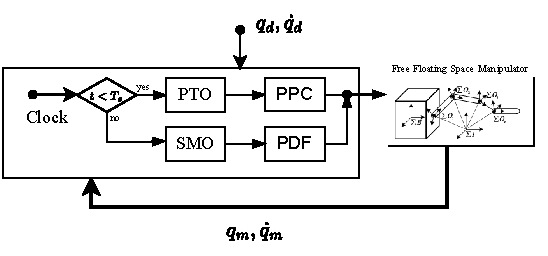
\includegraphics[width=0.8\textwidth]{assets/ppc-pdf.drawio.pdf}
  \caption{完整算法流程框图}
\end{figure}

\paragraph{(a) 可测的动量通道。}
由 \eqref{eq:model}，定义
\begin{equation}
y:=M_e(q_m)\dot q_m,\qquad
u_p:=\tau-C_e(q_m,\dot q_m)\dot q_m+\dot M_e(q_m,\dot q_m)\dot q_m,
\label{eq:momentum}
\end{equation}
其中 \(\dot M_e=\sum_{j}(\partial M_e/\partial q_{m,j})\dot q_{m,j}\) 由解析模型与可测的 \(q_m,\dot q_m\) 算出。由乘积法则与 \eqref{eq:model}，几乎处处有
\begin{equation}
\dot y=u_p+d(t).
\label{eq:momentum_channel}
\end{equation}
因此 \eqref{eq:momentum}--\eqref{eq:momentum_channel} 有两点用处：\textup{(i)} 观测不需要 \(\ddot q_m\)；\textup{(ii)} 被估计量直接是原扰动力矩 \(d\)，而不是 \(\Delta_a=M_e^{-1}d\)，故补偿量直接取 \(\hat d=z_2\) \eqref{eq:hatd}，不必再乘 \(M_e\)，且 \(d\) 为常值时并不要求 \(M_e\) 为常值。

\paragraph{(b) 观测器。}
取 \(\hat d=z_2\)，\(z_1,z_2\in\R^n\) 为观测器状态，\(\kappa_1,\kappa_2>0\) 为标量增益（逐分量可取不同值），\(\sig^{1/2}(s)=\lvert s\rvert^{1/2}\sgn(s)\) 逐分量定义：
\begin{equation}
\begin{cases}
\begin{aligned}
\dot z_1&=u_p+z_2+\dfrac{6}{T_o-t}\,(y-z_1),\\[2pt]
\dot z_2&=\dfrac{6}{(T_o-t)^{2}}\,(y-z_1),
\end{aligned}
&0\le t<T_o,\\[10pt]
\begin{aligned}
z_1(T_o)&:=\lim_{t\uparrow T_o}z_1(t)=y(T_o),\\
z_2(T_o)&:=\lim_{t\uparrow T_o}z_2(t)=d(T_o),
\end{aligned}
&t=T_o,\\[10pt]
\begin{aligned}
\dot z_1&=u_p+z_2+\kappa_1\sig^{1/2}(y-z_1),\\
\dot z_2&=\kappa_2\sgn(y-z_1),
\end{aligned}
&t>T_o,
\end{cases}
\label{eq:ptdo}
\end{equation}
\begin{equation}
\hat d(t)=z_2(t),\qquad t\ge0 .
\label{eq:hatd}
\end{equation}
\(T_o\) 处的等式是解的连续延拓（左极限），\emph{不是}需要在线获取 \(d(T_o)\) 的初始化指令：数值实现只需按上行积分至 \(T_o\)，随后以同一组状态继续积分下行，状态不重置、不改写。分段的分工是：上行利用 \(6/(T_o-t)\)、\(6/(T_o-t)^2\) 的奇异增益把误差在 \(T_o\) 处压到零；下行利用超螺旋结构把已经为零的误差锁在零上，且分母不再出现奇异项。

\paragraph{(c) 控制律。}
全时域力矩律仍取 \eqref{eq:computed_torque}（补偿量改为 \eqref{eq:hatd}），辅助输入按时段切换：
\begin{equation}
\nu(t)=
\begin{cases}
\nu^{\mathrm{PPC}}(t), & 0\le t<T_o,\\[2pt]
K_0z(t)-K_c(t-T_o)z(t-h), & t\ge T_o,
\end{cases}
\label{eq:nu_schedule}
\end{equation}
其中 \(z=[e^{\top},\dot e^{\top}]^{\top}\) 由 \eqref{eq:error_state} 给出，\(\nu^{\mathrm{PPC}}\) 由 \eqref{eq:nu_ppc} 给出，\(\rho_i\) 由 \eqref{eq:rho} 给出，\(K_0\in\R^{n\times2n}\) 使 \(A_c=A+BK_0\) Hurwitz，\(K_c\) 为 \eqref{eq:Kc} 给出的 \(2h\) 周期增益且在前半周期为零。由于 \(K_c(\vartheta)\equiv0\) 于 \(\vartheta\in[0,h)\)，延迟项只在 \(\vartheta\in[h,2h)\) 被激活，故只需缓存 \(t\ge T_o\) 之后 \(h\) 秒的 \(z\)，\emph{不需要}观测阶段的任何历史数据。

\paragraph{(d) 运行条件。}
算法的每条结论都由下列条件支撑，其中 \textup{(C1)(C2)} 只服务阶段 I，\textup{(C3)(C4)} 服务阶段 II，\textup{(C5)} 只服务“精确归零”。它们在假设~\ref{as:inertia}--\ref{as:observer}~下被逐条核验，此处集中列出以便复现：

\begin{enumerate}
\item[\textup{(C1)}] \textbf{模型与量测}：\(M_e\) 对称、连续可微、一致正定（\(\exists\underline m>0:\ M_e\succeq\underline m I_n\)），\(C_e(q_m,\dot q_m)\dot q_m\) 与 \eqref{eq:momentum} 中的 \(\dot M_e\dot q_m\) 精确可算；\(q_m,\dot q_m\) 可测，\emph{实际施加}的 \(\tau\) 已知；不需要 \(\ddot q_m\)。
\item[\textup{(C2)}] \textbf{阶段 I 扰动正则性}：\(d\) 在 \([0,T_o]\) 上绝对连续，且存在有限常数 \(L\) 使
\begin{equation}
\|\dot d(t)\|\le L\quad\text{对几乎所有 }t\in[0,T_o].
\label{eq:cond_L}
\end{equation}
\(L\) 的数值\emph{不}需要预先知道，只要求有限。
\item[\textup{(C3)}] \textbf{阶段 II 扰动正则性}：\(d\) 在 \([T_o,\infty)\) 上绝对连续，且逐分量存在有限常数 \(L_i,H_i\) 使
\begin{equation}
\lvert\dot d_i(t)\rvert\le L_i,\qquad
\lvert\ddot d_i(t)\rvert\le H_i
\quad\text{对几乎所有 }t\ge T_o,\ i=1,\dots,n .
\label{eq:cond_sta}
\end{equation}
\item[\textup{(C4)}] \textbf{超螺旋增益条件}：逐分量
\begin{equation}
\kappa_{2i}>L_i,\qquad
\kappa_{1i}^{2}>4L_i\,\frac{\kappa_{2i}+L_i}{\kappa_{2i}-L_i}.
\label{eq:cond_gain}
\end{equation}
它要求 \(L_i\) 已知（用于选增益）；例如取 \(\kappa_{2i}=2L_i\)、\(\kappa_{1i}=4\sqrt{L_i}\) 即满足 \eqref{eq:cond_gain}。不同文献对超螺旋的归一化不同，实施前须以同一约定核对 \eqref{eq:cond_gain}。
\item[\textup{(C5)}] \textbf{精确归零的理想前提}：连续时间实现、无执行器饱和、模型补偿精确（即假设~\ref{as:ideal}）。
\end{enumerate}

其中 \textup{(C2)} 只要求绝对连续且变化率有限，不要求概率模型、Lipschitz 常数已知或 \(d\) 逐点有界；\textup{(C3)} 是超螺旋保持零误差所需的正则性，比 \textup{(C2)} 强一阶，正是“\(T_o\) 前收敛、\(T_o\) 后保持”这一分段的代价。

\paragraph{(e) 时序。}
表~\ref{tab:schedule} 汇总完整算法的时间分段。总预设时间为 \(T_{\mathrm{pre}}=T_o+2h\)，只由设计参数给出。

\begin{table}[H]
\centering
\caption{完整算法的时间分段（观测器 \eqref{eq:ptdo}，辅助输入 \eqref{eq:nu_schedule}）}
\label{tab:schedule}
\small\begin{tabular}{llll}
\toprule
时段 & 观测器 & 辅助输入 & 该段承担的任务 \\
\midrule
\([0,T_o)\) & 上行（奇异增益） & \(\nu^{\mathrm{PPC}}\) \eqref{eq:nu_ppc} & \(z_2\to d(T_o)\)，包络 \(\lvert e_i\rvert<\rho_i\) \\
\(t=T_o\) & 左极限交接 & 允许跳变 & 进带 \(\lvert e_i(T_o)\rvert\le\vartheta_i\rho_{i\infty}\) \\
\([T_o,T_o+2h)\) & 下行（超螺旋） & \(K_0z-K_cz(t-h)\) & 单周期零化 \(z(T_o+2h)=0\) \\
\([T_o+2h,\infty)\) & 下行，误差恒零 & \(K_0z\) & 精确归零 \(e=\dot e=0\) \\
\bottomrule
\end{tabular}
\end{table}

\subsection{观测器：预设时刻收敛与超螺旋保持}
\label{sec:ptdo}

\paragraph{误差通道。}
由 \eqref{eq:computed_torque}、\eqref{eq:hatd} 与 \eqref{eq:model} 得
\begin{equation}
\ddot e=\nu+w,\qquad
w:=M_e^{-1}(q_m)\bigl[d-\hat d\bigr]=M_e^{-1}(q_m)\bigl[d-z_2\bigr],
\label{eq:decoupled_channel}
\end{equation}
即 \(w\) 是误差通道中唯一的未知输入。记 \(z=[e^{\top},\dot e^{\top}]^{\top}\)，\eqref{eq:decoupled_channel} 等价于
\begin{equation}
\dot z=Az+B\bigl(\nu+w\bigr),\qquad
A=\begin{bmatrix}0&I_n\\0&0\end{bmatrix},\quad B=\begin{bmatrix}0\\I_n\end{bmatrix}.
\label{eq:linear_error}
\end{equation}
于是观测任务可精确地表述为：使 \(w\) 在 \([0,T_o]\) 上\emph{有界}（阶段 I 的漏斗律只用到这一点），并使
\begin{equation}
w(t)\equiv0,\qquad \forall t\ge T_o
\label{eq:w_zero}
\end{equation}
成立（阶段 II 的线性延迟结构只用到这一点）。

\paragraph{阶段 I（\(0\le t<T_o\)）：奇异增益的预设时刻观测器。}
记
\begin{equation}
e_1=y-z_1,\qquad e_2=d-z_2,\qquad
x=\begin{bmatrix}e_1\\ (T_o-t)e_2\end{bmatrix},\qquad
\rho=\log\frac{T_o}{T_o-t},
\label{eq:obs_x}
\end{equation}
其中 \(\dd\rho/\dd t=1/(T_o-t)\)。由 \eqref{eq:momentum_channel} 与 \eqref{eq:ptdo} 上行得
\begin{equation}
\frac{\dd x}{\dd\rho}=A_o\,x+\begin{bmatrix}0\\ (T_o-t)^{2}\dot d\end{bmatrix},
\qquad
A_o=\begin{bmatrix}-6I_n&I_n\\-6I_n&-I_n\end{bmatrix},
\label{eq:obs_rho_dyn}
\end{equation}
而 \(A_o\) 的每个标量块的特征值为 \(-3,-4\)。即：在压缩时间坐标 \(\rho\) 下误差系统是\emph{定常}的，收缩率恒为 \(3\)；换回原时间坐标后 \(\rho\to\infty\) 当且仅当 \(t\uparrow T_o\)，故增益 \(6,6\) 的作用是把“指数收敛”平移为“在 \(T_o\) 时刻恰好收敛”。这一结构不需要 \(\lvert\dot d\rvert\) 的上界数值，只需其有限，因此 \(T_o\) 时刻的精度不依赖于对扰动的任何定量先验。增益对 \(6,6\) 的取法并非唯一：一般地取 \(r_1=3,r_2=4\)，则上行增益为 \(a_1=r_1+r_2-1=6\)、下行为 \(a_2=r_1r_2-a_1=6\)；改变 \((r_1,r_2)\) 会改变 \(A_o\) 的谱，但预设时刻性质不变。

\paragraph{阶段 II（\(t>T_o\)）：超螺旋滑模观测器。}
由 \eqref{eq:ptdo} 下行与 \eqref{eq:momentum_channel}，\eqref{eq:obs_x} 中的估计误差 \(e_1,e_2\) 满足
\begin{equation}
\dot e_1=e_2-\kappa_1\sig^{1/2}(e_1),\qquad
\dot e_2=\dot d-\kappa_2\sgn(e_1),
\label{eq:observer_errordyn}
\end{equation}
即标准的超螺旋误差系统。与常增益线性二阶观测器（其残差只能做到 \(O(L_+/\lambda)\)）不同，\eqref{eq:observer_errordyn} 在增益满足 \eqref{eq:cond_gain} 时具有滑模面 \(e_1=e_2=0\)：在滑模面上 \(\sgn(e_1)\) 的 Filippov 等效值自动取 \(\dot d/\kappa_2\)，把扰动的\emph{变化}实时抵消，因此 \(d\) 在 \(T_o\) 之后继续时变时估计仍然精确，而不仅是“误差足够小”。由于交接点已经给出 \(e_1(T_o)=e_2(T_o)=0\)（左极限），阶段 II 不需要到达过程，零误差在 \(T_o\) 之后被直接保持。

作为把观测结论接到控制结论上的桥，记阶段 I 的残差上界
\begin{equation}
\bar w:=\sup_{0\le t\le T_o}\bigl\lVert M_e^{-1}\bigl(d(t)-z_2(t)\bigr)\bigr\rVert_\infty<\infty ,
\label{eq:wbar_finite}
\end{equation}
它只度量阶段 I 的观测误差在加速度通道中的幅度，由定理~\ref{thm:ptdo_core}~(2) 给出显式上界。

\begin{theorem}[阶段 I：预设时间观测器]\label{thm:obs1}%
\label{thm:ptdo_core}\label{thm:ptdo}
设 \textup{(C1)} 成立，观测器取 \eqref{eq:ptdo} 上行，初始状态 \((z_1(0),z_2(0))\) 任意有限，估计误差按 \eqref{eq:obs_x} 定义。则：
\begin{enumerate}
  \item[\textup{(1)}] \textbf{预设时刻收敛}（需 \textup{(C2)}）：存在只由 \(A_o\) 决定的常数 \(K\ge1\)，使
\begin{equation}
\begin{aligned}
\|e_1(t)\|&\le K\|x(0)\|\Bigl(\frac{T_o-t}{T_o}\Bigr)^{3}
+KLT_o^{2}\Bigl[\Bigl(\frac{T_o-t}{T_o}\Bigr)^{2}-\Bigl(\frac{T_o-t}{T_o}\Bigr)^{3}\Bigr],\\
\|e_2(t)\|&\le\frac{K\|x(0)\|}{T_o}\Bigl(\frac{T_o-t}{T_o}\Bigr)^{2}
+KL\Bigl[(T_o-t)-\frac{(T_o-t)^{2}}{T_o}\Bigr],
\end{aligned}
\label{eq:observer_bounds}
\end{equation}
从而 \(\lim_{t\uparrow T_o}z_1(t)=y(T_o)\)、\(\lim_{t\uparrow T_o}z_2(t)=d(T_o)\)。收敛时刻恰为 \(T_o\)：是否收敛只取决于 \(\lVert x(0)\rVert<\infty\) 与 \(L<\infty\)，与二者的数值无关（\eqref{eq:observer_bounds}~本身含二者的数值）。
  \item[\textup{(2)}] \textbf{阶段 I 残差界}（需 \textup{(C1)(C2)}）：\eqref{eq:wbar_finite} 中的 \(\bar w\) 可显式取为
\begin{equation}
\bar w\le\frac{1}{\underline m}\Bigl[\frac{K\|x(0)\|}{T_o}+\frac{KLT_o}{4}\Bigr],
\label{eq:residual_bound}
\end{equation}
其中 \(\underline m\) 为 \(M_e\) 的正定下界，\(x(0)\) 由 \eqref{eq:obs_x} 给出。
\end{enumerate}
\end{theorem}

\begin{proof}
\textbf{(1)} 由 \eqref{eq:momentum_channel} 与 \eqref{eq:ptdo} 上行，
\begin{equation}
\dot e_1=e_2-\frac{6}{T_o-t}e_1,\qquad
\dot e_2=\dot d(t)-\frac{6}{(T_o-t)^{2}}e_1 .
\label{eq:obs_err_time}
\end{equation}
右端在 \([0,T_o)\) 上关于 \(t\) 局部有界（\(e_1,e_2\) 连续、\(\dot d\) 有界），故对任意有限初值，解在 \([0,T_o)\) 上存在唯一且绝对连续。以 \eqref{eq:obs_x} 的 \(x\) 与压缩时间 \(\rho=\log\frac{T_o}{T_o-t}\) 为坐标，注意 \(\dd t/\dd\rho=T_o-t\)，由 \eqref{eq:obs_err_time} 得 \eqref{eq:obs_rho_dyn}：其第一行为
\[
\frac{\dd x_1}{\dd\rho}=(T_o-t)\dot e_1=(T_o-t)e_2-6e_1=x_2-6x_1 ,
\]
第二行对 \(x_2=(T_o-t)e_2\) 求导（注意 \(\dd(T_o-t)/\dd\rho=-(T_o-t)\)）得 \([-6,-1]\) 与强迫项 \((T_o-t)^{2}\dot d\)。\(A_o\) 的标量块 \(\begin{bmatrix}-6&1\\-6&-1\end{bmatrix}\) 的特征多项式为 \(\lambda^{2}+7\lambda+12=(\lambda+3)(\lambda+4)\)，两特征值互异，故 \(A_o\) 可对角化；存在 \(K\ge1\)（取 \(K=\lVert V\rVert\lVert V^{-1}\rVert\)，\(V\) 为特征向量矩阵）使
\[
\bigl\lVert e^{A_o\rho}\bigr\rVert\le Ke^{-3\rho}=K\Bigl(\frac{T_o-t}{T_o}\Bigr)^{3}.
\]
又 \(\bigl\lVert[0,\ (T_o-t)^{2}\dot d]^{\top}\bigr\rVert\le LT_o^{2}e^{-2\rho}\)。由 \eqref{eq:obs_rho_dyn} 的常数变易公式，
\[
\lVert x(\rho)\rVert\le Ke^{-3\rho}\lVert x(0)\rVert
+\int_0^{\rho}Ke^{-3(\rho-s)}LT_o^{2}e^{-2s}\dd s
=K\lVert x(0)\rVert r^{3}+KLT_o^{2}(r^{2}-r^{3}),
\]
其中 \(r:=(T_o-t)/T_o=e^{-\rho}\in(0,1]\)，并用到 \(\int_0^{\rho}e^{-3(\rho-s)}e^{-2s}\dd s=e^{-2\rho}-e^{-3\rho}\)。再由 \(\lVert e_1\rVert=\lVert x_1\rVert\le\lVert x\rVert\) 与 \(\lVert e_2\rVert=\lVert x_2\rVert/(T_o-t)\) 即得 \eqref{eq:observer_bounds}。令 \(t\uparrow T_o\)（即 \(r\to0\)），两式右端均趋于零，故 \(e_1,e_2\to0\)，即 \(z_1\to y(T_o)\)、\(z_2\to d(T_o)\)。

\textbf{(2)} 由 \(w=M_e^{-1}(d-z_2)=M_e^{-1}e_2\) 与 \(\lVert M_e^{-1}\rVert_2\le1/\underline m\)，
\[
\lVert w(t)\rVert_2\le\frac{1}{\underline m}
\Bigl[\frac{K\lVert x(0)\rVert}{T_o}r^{2}
+K\Bigl((T_o-t)-\frac{(T_o-t)^{2}}{T_o}\Bigr)L\Bigr].
\]
其中 \(r^{2}\le1\)，而 \(s(T_o-s)/T_o\)（\(s=T_o-t\in[0,T_o]\)）在 \(s=T_o/2\) 处取最大值 \(T_o/4\)。故 \eqref{eq:residual_bound} 成立（若 \(\bar w\) 按 \eqref{eq:wbar_finite} 的 \(\lVert\cdot\rVert_\infty\) 定义，则右端再乘一个仅依赖维数 \(n\) 的常数，结论不变）。
\end{proof}

\begin{remark}[交接点与残差的含义]\label{rem:handover_obs}
定理~\ref{thm:ptdo_core}~(1) 的界依赖于 \(\|x(0)\|\)，其中 \(e_2(0)=d(0)-z_2(0)\) 含未知的 \(d(0)\)；该量只用于给出\emph{界}，实现时并不需要知道它——观测器初值可由 \(z_2(0)=0\) 任意取定，界随之变松但不影响“在 \(T_o\) 收敛”这一结论。定理~\ref{thm:ptdo_core}~(2) 是把该界换算到加速度通道 \(w\) 的结果，它给出阶段 I 漏斗律所需的 \(\bar w\)：\eqref{eq:residual_bound} 关于 \(T_o\) 呈 \(A/T_o+BT_o\) 形，存在折中最优，这与第~\ref{sec:algorithm}~节关于 \(T_o\) 的整定讨论一致。
\end{remark}

\begin{lemma}[超螺旋有限时间收敛]\label{lem:sta}
考虑标量误差系统
\begin{equation}
\dot e_1=e_2-\kappa_1\lvert e_1\rvert^{1/2}\sgn(e_1),\qquad
\dot e_2=\rho(t)-\kappa_2\sgn(e_1),
\label{eq:sta_scalar}
\end{equation}
其中 \(\rho\) 可测且逐点满足 \(\lvert\rho(t)\rvert\le L\)。若
\begin{equation}
\kappa_2>L,\qquad \kappa_1^{2}>4L\,\frac{\kappa_2+L}{\kappa_2-L},
\label{eq:sta_gain}
\end{equation}
则 \eqref{eq:sta_scalar} 的每个 Filippov 解在有限时间内到达原点并此后保持；特别地，若 \(e_1(t_0)=e_2(t_0)=0\)，则 \(e_1(t)=e_2(t)=0\) 对一切 \(t\ge t_0\)。
\end{lemma}

\begin{proof}
取强 Lyapunov 函数\cite{moreno2012strict}
\[
\zeta=\begin{bmatrix}\lvert e_1\rvert^{1/2}\sgn(e_1)\\ e_2\end{bmatrix},\qquad
P=\frac12\begin{bmatrix}4\kappa_2+\kappa_1^{2}&-\kappa_1\\-\kappa_1&2\end{bmatrix},\qquad
V=\zeta^{\top}P\zeta .
\]
由 \(\kappa_2>L\ge0\) 知 \(P\succ0\)，且存在 \(0<a\le b\) 使 \(a\lVert\zeta\rVert^{2}\le V\le b\lVert\zeta\rVert^{2}\)。沿 \eqref{eq:sta_scalar} 在 \(e_1\ne0\) 处求导并利用 \(\lvert\rho\rvert\le L\)，直接计算得
\[
\dot V\le-\frac{1}{\lvert e_1\rvert^{1/2}}\,\zeta^{\top}Q\,\zeta ,
\]
其中对称阵 \(Q\) 正定当且仅当 \eqref{eq:sta_gain} 成立（Moreno--Osorio 判据）。于是存在 \(c>0\) 使 \(\dot V\le-cV^{1/2}\)，从而
\[
V^{1/2}(t)\le V^{1/2}(t_0)-\frac{c}{2}(t-t_0),
\]
解在 \(T\le t_0+2V^{1/2}(t_0)/c\) 内到达 \(V=0\)，即 \(e_1=e_2=0\)。在原点处 Filippov 集包含零：由 \(\lvert\rho\rvert\le L<\kappa_2\) 可取 \(\sgn(0)=\rho/\kappa_2\in[-1,1]\)，故原点是 Filippov 解的不变集。于是若 \(V(t_0)=0\)，上式给出 \(V(t)\equiv0\) 于 \(t\ge t_0\)。
\end{proof}

\begin{theorem}[阶段 II：超螺旋滑模观测器]\label{thm:obs2}%
\label{thm:sta}
设 \textup{(C1)(C3)(C4)} 成立，\(t\ge T_o\) 的观测器取 \eqref{eq:ptdo} 下行，且 \(T_o\) 处的初值取定理~\ref{thm:obs1}~(1) 的左极限，即 \(e_1(T_o)=e_2(T_o)=0\)。则对一切 \(t\ge T_o\)
\begin{equation}
e_1(t)=e_2(t)=0,\qquad z_2(t)=d(t),\qquad \hat d(t)=d(t),
\label{eq:observer_converged}
\end{equation}
等价地 \eqref{eq:w_zero} 成立；即阶段 II 的通道无扰动，且该结论对 \(t\ge T_o\) 上继续时变的 \(d\) 同样成立。若交接处存在有界失配 \(e_1(T_o),e_2(T_o)\neq0\)，误差仍在有限时间内到达零并保持。
\end{theorem}

\begin{proof}
由 \eqref{eq:ptdo} 下行与 \eqref{eq:momentum_channel} 得 \eqref{eq:observer_errordyn}，其逐分量为 \eqref{eq:sta_scalar} 的形式，不确定项为 \(\rho=\dot d_i\)，由 \textup{(C3)} 有 \(\lvert\dot d_i\rvert\le L_i\)。\textup{(C4)} 的 \eqref{eq:cond_gain} 逐分量给出引理~\ref{lem:sta} 的条件 \eqref{eq:sta_gain}。由交接条件 \(e_1(T_o)=e_2(T_o)=0\)，引理~\ref{lem:sta} 给出 \(e_1=e_2=0\) 于 \([T_o,\infty)\)；代入 \(e_2=d-z_2\) 及 \eqref{eq:hatd}、\eqref{eq:decoupled_channel} 即得 \eqref{eq:observer_converged} 与 \eqref{eq:w_zero}。时变扰动只通过界 \(L_i\) 进入增益条件，故对 \(t\ge T_o\) 上继续时变的 \(d\) 同样成立；若交接失配非零，引理~\ref{lem:sta} 的有限时间收敛部分给出到达时刻 \(T_o+2\max_iV_i^{1/2}(T_o)/c_i\)（\(V_i,c_i\) 为引理~\ref{lem:sta} 证明中的 Lyapunov 量与收缩常数），此后保持为零。
\end{proof}

\begin{remark}[为何不在 \(T_o\) 后继续用线性观测器]\label{rem:sta_vs_linear}
若把 \eqref{eq:ptdo} 的下行换成常增益线性结构 \(\dot z_1=u_p+z_2+2\lambda(y-z_1)\)、\(\dot z_2=\lambda^{2}(y-z_1)\)，则由 \eqref{eq:observer_errordyn} 的线性对应可得 \(\|e_2(t)\|\le (L_+/\lambda)[2-(2+\lambda h)e^{-\lambda h}]\)，即只有 \(O(L_+/\lambda)\) 的残差，\(d\) 时变时\emph{不能}保持零误差；增大 \(\lambda\) 虽缩小残差，却同时放大噪声与离散抖振。超螺旋结构的价值正在于把这一“残差随 \(L_+\) 线性恶化”的结论替换为“在 \eqref{eq:cond_gain} 下严格为零”，代价是要求 \(d\) 的二阶导数有界 \textup{(C3)} 与 \(\sgn\) 带来的抖振（第~\ref{sec:infeasible}~节）。
\end{remark}

\subsection{阶段 I：漏斗型预设性能律}
\label{sec:ppc}

取 \(\xi_i=e_i/\rho_i\in(-1,1)\)，并由可测量构造
\begin{equation}
\dot\xi_i=\frac{\dot e_i-\xi_i\dot\rho_i}{\rho_i},\qquad
s_i=\dot\xi_i+k_{1i}\xi_i,\qquad k_{1i}>0 ,
\label{eq:xi_s}
\end{equation}
及控制律
\begin{equation}
\nu_i^{\mathrm{PPC}}=\rho_i\Bigl[-k_{2i}s_i-\frac{\xi_i}{1-\xi_i^{2}}-k_{1i}\dot\xi_i\Bigr]
+\ddot\rho_i\,\xi_i+2\dot\rho_i\,\dot\xi_i,\qquad k_{2i}>0 .
\label{eq:nu_ppc}
\end{equation}
方括号内为漏斗反步项，其中 \(-\xi_i/(1-\xi_i^2)\) 是障碍项，其系数必须取 \(1\) 才能与 \(\xi\) 动力学中的交叉项精确相消；\(\ddot\rho_i\xi_i\) 与 \(2\dot\rho_i\dot\xi_i\) 是时变归一化引起的虚拟强迫项。由引理~\ref{lem:rho_smooth}，\(\rho_i,\dot\rho_i,\ddot\rho_i\) 均为已知时间函数，故 \eqref{eq:xi_s}、\eqref{eq:nu_ppc} 仅依赖测量。

该律的闭环性质由定理~\ref{thm:ppc} 给出。为此只需引入以下量：由 \eqref{eq:decoupled_channel} 降阶后的候选 Lyapunov 函数，以及由 \eqref{eq:residual_bound} 的 \(\bar w\) 决定的常数
\begin{equation}
V_i=\tfrac12\ln\frac{1}{1-\xi_i^{2}}+\tfrac12 s_i^{2},\quad
\bar V_i=\tfrac12\ln\frac{c_i+k_{1i}}{k_{1i}}+\frac{c_i}{k_{2i}},\quad
c_i=\frac{\sigma_i^{2}}{2k_{2i}},\quad
\sigma_i=\frac{\bar w}{\rho_{i\infty}} ;
\label{eq:V_c}
\end{equation}
\begin{theorem}[阶段 I：漏斗型预设性能控制]\label{thm:ppc}\label{thm:funnel}
设 \textup{(C1)(C2)} 成立，\(\bar w\) 由 \eqref{eq:residual_bound} 取定（有限），性能函数取 \eqref{eq:rho}，辅助输入取 \eqref{eq:nu_ppc}，初值满足假设~\ref{as:ic}（即 \(\lvert\xi_i(0)\rvert<1\)）。则闭环在 \([0,T_o]\) 上无有限时刻逃逸，且
\begin{enumerate}
  \item[\textup{(1)}] \textbf{一致界与包络}：
\begin{equation}
\lvert e_i(t)\rvert\le\vartheta_i\rho_i(t)<\rho_i(t),\qquad
\vartheta_i=\sqrt{1-e^{-2\max\{V_i(0),\bar V_i\}}}<1,
\label{eq:funnel_bound}
\end{equation}
对一切 \(t\in[0,T_o]\) 与 \(i=1,\dots,n\)，其中 \(V_i,\bar V_i\) 由 \eqref{eq:V_c} 给出；\(\vartheta_i<1\) 对任意\emph{有限} \(\bar w\) 成立，与 \(\bar w\) 的数值无关。
  \item[\textup{(2)}] \textbf{进带}（第一预设时间）：\(\lvert e_i(T_o)\rvert\le\vartheta_i\rho_{i\infty}<\rho_{i\infty}\)。
\end{enumerate}
\end{theorem}

\begin{proof}
\textbf{第 1 步（降阶）。}由 \(\dot e_i=\dot\rho_i\xi_i+\rho_i\dot\xi_i\)、\(\ddot e_i=\ddot\rho_i\xi_i+2\dot\rho_i\dot\xi_i+\rho_i\ddot\xi_i\) 与 \eqref{eq:decoupled_channel} 得 \(\ddot\xi_i=(\nu_i+w_i-\ddot\rho_i\xi_i-2\dot\rho_i\dot\xi_i)/\rho_i\)。对其与 \eqref{eq:xi_s} 求导后代入 \eqref{eq:nu_ppc}，前馈项精确相消，得
\begin{equation}
\dot\xi_i=s_i-k_{1i}\xi_i,\qquad
\dot s_i=-k_{2i}s_i-\frac{\xi_i}{1-\xi_i^{2}}+\frac{w_i}{\rho_i}.
\label{eq:s_dyn}
\end{equation}

\textbf{第 2 步（Lyapunov 一致界）。}沿 \eqref{eq:s_dyn}，
\begin{equation}
\dot V_i=\frac{\xi_i\dot\xi_i}{1-\xi_i^{2}}+s_i\dot s_i
=-\frac{k_{1i}\xi_i^{2}}{1-\xi_i^{2}}-k_{2i}s_i^{2}+\frac{s_iw_i}{\rho_i},
\label{eq:Vdot}
\end{equation}
交叉项 \(\xi_is_i/(1-\xi_i^2)\) 精确相消。由 \(\rho_i\ge\rho_{i\infty}\)、\(\lvert w_i\rvert\le\bar w\) 得 \(\lvert w_i\rvert/\rho_i\le\sigma_i=\bar w/\rho_{i\infty}\)，用 Young 不等式 \(\lvert s_i\rvert\sigma_i\le\frac12k_{2i}s_i^2+\frac{\sigma_i^2}{2k_{2i}}\) 得
\begin{equation}
\dot V_i\le-\frac{k_{1i}\xi_i^{2}}{1-\xi_i^{2}}-\frac{k_{2i}}{2}s_i^{2}+c_i .
\label{eq:Vdot_bound}
\end{equation}
记 \(\Omega_i=\{(\xi_i,s_i):\dot V_i\ge0\}\)。由 \eqref{eq:Vdot_bound}，在 \(\Omega_i\) 上 \(k_{1i}\xi_i^2/(1-\xi_i^2)\le c_i\) 且 \(\frac{k_{2i}}{2}s_i^2\le c_i\)，前者等价于 \(\lvert\xi_i\rvert\le\bar\xi_i=\sqrt{c_i/(c_i+k_{1i})}<1\)，即 \(\Omega_i\) 严格位于开集 \(\{\lvert\xi_i\rvert<1\}\) 内。于是 \(\Omega_i\) 上 \(V_i\le\frac12\ln\frac{1}{1-\bar\xi_i^2}+\frac{c_i}{k_{2i}}=\bar V_i\)，从而 \(\dot V_i\le0\) 与 \(V_i\le\bar V_i\) 同时成立。在 \(V_i\) 首次超过 \(\max\{V_i(0),\bar V_i\}\) 的时刻取反证，得
\begin{equation}
V_i(t)\le V_i^{\max}:=\max\{V_i(0),\bar V_i\},\qquad\forall t\in[0,T_o]\ \text{（只要解存在）}.
\label{eq:Vmax}
\end{equation}

\textbf{第 3 步（无逃逸与进带）。}\eqref{eq:nu_ppc} 右端在开集 \(\{\lvert\xi_i\rvert<1\}\times\R\) 上局部 Lipschitz（\(\rho_i^{(\cdot)}\) 连续，\(\lvert\xi_i\rvert<1\) 时 \(1-\xi_i^2>0\)），故局部解存在唯一。设 \(t^\ast\) 为首次满足 \(\lvert\xi_i\rvert=1\) 的时刻，则在 \([0,t^\ast)\) 上由 \eqref{eq:Vmax} 得 \(\frac12\ln\frac{1}{1-\xi_i^2}\le V_i^{\max}\)，即 \(\lvert\xi_i\rvert\le\sqrt{1-e^{-2V_i^{\max}}}<1\)，与 \(\lvert\xi_i(t^\ast)\rvert=1\) 矛盾，故 \(t^\ast=+\infty\) 且 \eqref{eq:funnel_bound} 成立，此即 (1)。代入 \(t=T_o\)、\(\rho_i(T_o)=\rho_{i\infty}\) 得 (2)。又 \(c_i<\infty\) 蕴含 \(\bar V_i<\infty\) 与 \(\vartheta_i<1\)，故 (1)(2) 与 \(\bar w\) 的取值无关。
\end{proof}

障碍增益取 \(1\) 的必要性在于：它使 \eqref{eq:s_dyn} 的交叉项 \(\xi_is_i/(1-\xi_i^2)\) 在 \(\dot V_i\) 中\emph{精确}相消，故包络的结构性成立不依赖 \(\bar w\) 的数值。

\subsection{阶段 II：Gramian 型周期延迟反馈}
\label{sec:pdf}

以局部时间 \(\vartheta=t-T_o\) 重新计时。由 \eqref{eq:w_zero}，\eqref{eq:linear_error}~在 \(\vartheta\ge0\) 上严格线性，取
\begin{equation}
\nu(\vartheta)=K_0z(\vartheta)-K_c(\vartheta)z(\vartheta-h),\qquad
K_c(\vartheta)=0\ (\vartheta\in[0,h)),
\label{eq:pdf_input}
\end{equation}
得闭环延迟系统 \(\dot z=A_cz(\vartheta)-BK_c(\vartheta)z(\vartheta-h)\)。取 \(2h\) 周期光滑函数 \(R_h\ge0\)（\(R_h\equiv0\) 于 \([0,h]\)，在每个 \([h,2h]\) 上的某正测度子集上严格正），定义
\begin{equation}
W_c=\int_h^{2h}e^{-A_cs}BR_h(s)B^{\top}e^{-A_c^{\top}s}\dd s\succ0 .
\label{eq:Wc}
\end{equation}
由 \(\vartheta\ge0\) 上通道 \eqref{eq:linear_error} 中 \((A,B)\) 的可控性（\(\operatorname{rank}[B,AB]=2n\)）与 \(K_0\) 的极点配置知 \((A_c,B)\) 可控，结合 \(R_h\) 的支撑条件得 \(W_c\succ0\)。增益取
\begin{equation}
K_c(\vartheta)=
\begin{cases}
0, & \vartheta\in[0,h),\\[2pt]
R_h(\vartheta)B^{\top}e^{-A_c^{\top}\vartheta}W_c^{-1}e^{A_c(h-\vartheta)}, & \vartheta\in[h,2h),
\end{cases}
\label{eq:Kc}
\end{equation}
并以 \(2h\) 周期延拓。记闭环 \(\dot z=A_cz(\vartheta)-BK_c(\vartheta)z(\vartheta-h)\) 在 \([0,2h]\) 上的单周期状态转移矩阵为 \(\Delta_K(h)\)；设计目标是使 \(\Delta_K(h)=0\)，它与由此得到的永久零化由下面的定理~\ref{thm:pdf1} 给出。

\begin{theorem}[阶段 II：预设时间 PDF 控制]\label{thm:pdf1}\label{thm:pdf}
设 \(\vartheta\ge0\) 上通道严格为 \eqref{eq:linear_error}（即 \(w\equiv0\)，见 \eqref{eq:w_zero}），辅助输入取 \eqref{eq:pdf_input}，\(K_c\) 由 \eqref{eq:Kc} 给出，\(R_h\) 满足支撑条件且 \(W_c\succ0\)。则
\begin{enumerate}
  \item[\textup{(1)}] \textbf{单周期零化}：\(\Delta_K(h)=0\)；
  \item[\textup{(2)}] \textbf{永久零化}（第二预设时间）：对任意有界初值 \(z(T_o)\)，闭环解满足
\[
z(\vartheta)=0,\quad\forall\vartheta\ge2h,
\qquad\text{即}\quad e(t)=\dot e(t)=0,\quad\forall t\ge T_o+2h .
\]
\end{enumerate}
结论不要求 \(\nu\) 在 \(T_o\) 处连续：切换跳变只改变 \(\nu\) 的取值，不改变以 \(z(T_o)\) 为初值的线性系统的解。
\end{theorem}

\begin{proof}
\textbf{(1)} 前段 \(\vartheta\in[0,h]\)：\(K_c=0\)，\(z(\vartheta)=e^{A_c\vartheta}z(0)\)，故 \(z(h)=e^{A_ch}z(0)\) 且 \(\vartheta\in[h,2h]\) 时 \(z(\vartheta-h)=e^{A_c(\vartheta-h)}z(0)\)。后段由变分公式
\[
z(2h)=e^{A_c2h}z(0)-\int_h^{2h}e^{A_c(2h-s)}BK_c(s)e^{A_c(s-h)}\dd s\,z(0).
\]
注意 \(e^{A_c(h-s)}e^{A_c(s-h)}=I_{2n}\) 与 \(e^{A_c(2h-s)}=e^{A_c2h}e^{-A_cs}\)，代入 \eqref{eq:Kc} 得
\[
\int_h^{2h}e^{A_c(2h-s)}BK_c(s)e^{A_c(s-h)}\dd s
=e^{A_c2h}\int_h^{2h}e^{-A_cs}BR_hB^{\top}e^{-A_c^{\top}s}\dd s\,W_c^{-1}=e^{A_c2h},
\]
故 \(\Delta_K(h)=0\)。（此处 \(z(0)\) 指局部时间起点处的状态，即 \(z(T_o)\)。）

\textbf{(2)} \(\vartheta\in[2h,3h)\) 时 \(K_c=0\)，\(\dot z=A_cz\) 且 \(z(2h)=0\)，故 \(z\equiv0\)；\(\vartheta\in[3h,4h)\) 时 \(K_c\neq0\) 但 \(z(\vartheta-h)=0\)，仍为 \(\dot z=A_cz\) 且 \(z(3h)=0\)。逐周期归纳得 \(z(\vartheta)=0\) 于 \(\vartheta\ge2h\)；由 \eqref{eq:linear_error} 回代 \(t=T_o+\vartheta\) 即得 \(e(t)=\dot e(t)=0\) 于 \(t\ge T_o+2h\)。
\end{proof}

\subsection{四个分定理及其合成}
\label{sec:algo_proof}

按时间轴，上面四个分定理各管一段，其依赖关系如下：
\begin{itemize}
  \item 定理~\ref{thm:obs1}（\(T_o\) 前预设时间观测）：\textup{(C1)(C2)} \(\Rightarrow\) \eqref{eq:observer_bounds} 与残差界 \eqref{eq:residual_bound}；
  \item 定理~\ref{thm:sta}（\(T_o\) 后滑模观测）：\textup{(C3)(C4)} 与左极限交接 \(\Rightarrow\) \eqref{eq:observer_converged}，即 \(w\equiv0\) 于 \(t\ge T_o\)；
  \item 定理~\ref{thm:ppc}（\(T_o\) 前 PPC）：\textup{(C1)(C2)} 与 \eqref{eq:residual_bound} 的 \(\bar w\) \(\Rightarrow\) 包络 \eqref{eq:funnel_bound} 与进带；
  \item 定理~\ref{thm:pdf1}（\(T_o\) 后 PDF）：\(w\equiv0\) 与 \(\Delta_K(h)=0\) \(\Rightarrow\) \(z(\vartheta)=0\) 于 \(\vartheta\ge2h\)。
\end{itemize}
四个分定理的合成给出第~\ref{sec:analysis}~节的\emph{总定理}（定理~\ref{thm:main}）：\textup{(C1)(C2)} 承担包络、进带与阶段 I 观测；\textup{(C3)(C4)} 把阶段 II 的通道化为无扰动；\textup{(C5)} 与 \(\Delta_K(h)=0\) 完成精确归零。合成只需要一个连接量——交接状态界 \(\lVert z(T_o)\rVert\le B_o\)（引理~\ref{lem:handover}），它把定理~\ref{thm:ppc}~(1) 的包络估计接到定理~\ref{thm:pdf1} 的线性算子上。四段时长为 \(T_o\)（观测与包络）、\(h\)（纯 \(A_c\) 传播）与 \(h\)（注入—抵消），故总预设时间 \(T_{\mathrm{pre}}=T_o+2h\)，只由设计参数给出。

\begin{remark}[“不需要扰动上界”的确切含义]\label{rem:unknown_w}
定理~\ref{thm:ppc}~(1)(2) 的结论分两层：\emph{包络成立性}只要求 \(\bar w\) 有限（定理~\ref{thm:ppc} 第 2 步中 \(c_i<\infty\)），故即便不知 \(\bar w\) 包络也不破；\emph{贴合深度} \(\vartheta_i\) 的数值依赖 \(\bar w\)（\(c_i\propto\bar w^2\)，\(\bar w\to\infty\) 时 \(\vartheta_i\to1\)）。即未知扰动幅度只消耗误差带内部余量，不破坏结构保证；但整定与验收仍需一个保守估计（可由 \eqref{eq:residual_bound} 给出，其中 \(L\) 可离线估计而无需在线测量）。
\end{remark}

\begin{remark}[障碍增益与饱和]\label{rem:barrier}
障碍项在 \(\lvert\xi_i\rvert\to1\) 时发散，这是包络\emph{结构性}成立的原因（定理~\ref{thm:ppc} 证明第 3 步的反证），也使初始点靠近包络时力矩峰值增大；若改用纯误差变换实现（不加障碍项），输入保持有界但有界性论证需引入 \(S'\) 的下界估计、鲁棒性变差。故保留障碍型实现，饱和下的降级见第~\ref{sec:infeasible}~节。
\end{remark}

\subsection{完整算法与参数约束}
\label{sec:algorithm}

实现流程为：\textbf{(1)} 选定 \(T_o\)、\(\rho_{i0}>\rho_{i\infty}>0\)（本文固定五次多项式）；\textbf{(2)} 选定 \(k_{1i},k_{2i}\) 并按推论~\ref{cor:exponential}~校验 \(2\underline k_iT_o\gtrsim\ln(\rho_{i0}/\rho_{i\infty})\)；\textbf{(3)} 选定超螺旋增益 \(\kappa_{1i},\kappa_{2i}\) 并核验 \textup{(C3)(C4)}，即 \eqref{eq:cond_sta}--\eqref{eq:cond_gain}（\(L_i\) 须先由扰动包络离线估计）；同时核验 \textup{(C2)} 的 \(L<\infty\)，并由 \eqref{eq:residual_bound} 算出阶段 I 的 \(\bar w\)，用于 \eqref{eq:V_c} 与 \eqref{eq:B_o}；\textbf{(4)} 选定 \(K_0,h,R_h\)，数值积分 \(W_c\)（正则化求逆只给近似零化，不满足定理~\ref{thm:main}~(iv) 的精确归零前提）；\textbf{(5)} \textbf{校验} \(\lVert\Delta_K(h)\rVert\) 与 \(\operatorname{cond}(W_c)\)，若不达标返回 (4)；\textbf{(6)} 由命题~\ref{prop:stage2}~算 \(M_h\) 并校验包络交接。第 (5) 步是算法可靠性的必要环节：若数值精度使 \(\Delta_K(h)\neq0\)，结论退化为命题~\ref{prop:approx}；若 \(\lVert\Delta_K(h)\rVert\ge1\)，连有界性都无法由该递推得到（第~\ref{sec:infeasible}~节）。

参数耦合须成对检查：增益增大使 \(\vartheta_i\) 减小但力矩峰值上升；误差带收窄使 \(\sigma_i=\bar w/\rho_{i\infty}\) 增大、\(\vartheta_i\to1\)，边际收益递减；\(T_o\) 减小使 \(\dot\rho_i\propto1/T_o\) 增大而力矩上升、增大则残差界 \eqref{eq:residual_bound} 中的 \(KLT_o/4\) 项增大，故存在折中最优；\(h\) 减小使归零更快但 \(W_c\) 条件数恶化；\(\kappa_{1i},\kappa_{2i}\) 只能由 \(L_i\) 从下方约束（\eqref{eq:cond_gain}），取得过大虽仍保持零误差，却会放大 \(\sgn\) 的离散抖振与力矩峰值。

\section{闭环性能分析}
\label{sec:analysis}

\subsection{交接状态与总定理}
\label{sec:main}

\begin{lemma}[交接状态有界]\label{lem:handover}
在定理~\ref{thm:ppc}~(1) 的条件下，
\begin{equation}
\lVert z(T_o)\rVert\le B_o:=\Bigl(\sum_{i}\vartheta_i^2\rho_{i\infty}^{2}
+\sum_{i}\rho_{i\infty}^{2}\bigl(\sqrt{2V_i^{\max}}+k_{1i}\bigr)^{2}\Bigr)^{1/2}.
\label{eq:B_o}
\end{equation}
\end{lemma}

\begin{proof}
由 \eqref{eq:funnel_bound} 得 \(\lvert e_i(T_o)\rvert\le\vartheta_i\rho_{i\infty}\)。又 \(\dot e_i=\dot\rho_i\xi_i+\rho_i\dot\xi_i\)，\(\lvert\dot\xi_i\rvert\le\lvert s_i\rvert+k_{1i}\lvert\xi_i\rvert\le\sqrt{2V_i^{\max}}+k_{1i}\)，而 \(\dot\rho_i(T_o)=0\)，故 \(\lvert\dot e_i(T_o)\rvert\le\rho_{i\infty}(\sqrt{2V_i^{\max}}+k_{1i})\)。
\end{proof}

\begin{theorem}[总定理：双重预设时间跟踪]\label{thm:main}\label{thm:algo}
设假设~\ref{as:inertia}--\ref{as:observer}~成立，并记 \textup{(C1)}--\textup{(C5)} 如第~\ref{sec:structure}~节所述。取力矩律 \eqref{eq:computed_torque}、\eqref{eq:hatd}（\(\hat d=z_2\)）、观测器 \eqref{eq:ptdo}、辅助输入 \eqref{eq:nu_schedule}（\(\nu^{\mathrm{PPC}}\) 由 \eqref{eq:nu_ppc}、\(K_c\) 由 \eqref{eq:Kc} 给出）、性能函数 \eqref{eq:rho}，并设 \(\Delta_K(h)=0\)。则下面的结论分别由四个分定理给出、并在本定理中合成为一个闭环结论：
\begin{enumerate}
  \item[(i)] \textbf{包络}（\(T_o\) 前，\textup{(C1)(C2)}；定理~\ref{thm:ppc}~(1)）：\(\lvert e_i(t)\rvert\le\vartheta_i\rho_i(t)<\rho_i(t)\)，\(\forall t\in[0,T_o]\)；
  \item[(ii)] \textbf{进带}（第一预设时间，\textup{(C1)(C2)}；定理~\ref{thm:ppc}~(2)）：\(\lvert e_i(T_o)\rvert\le\vartheta_i\rho_{i\infty}<\rho_{i\infty}\)；
  \item[(iii)] \textbf{过渡}（PDF 驱动阶段，\textup{(C3)(C4)}；定理~\ref{thm:sta}）：\(\lvert e_i(t)\rvert\le M_{h,i}B_o\)，\(\forall t\in[T_o,T_o+2h)\)，\(M_{h,i}\) 见 \eqref{eq:Mh}；
  \item[(iv)] \textbf{归零}（第二预设时间，\textup{(C5)} 与 \(\Delta_K(h)=0\)；定理~\ref{thm:pdf1}~(2)）：\(e(t)=\dot e(t)=0\)，\(\forall t\ge T_o+2h\)。
\end{enumerate}
总预设时间 \(T_{\mathrm{pre}}=T_o+2h\)，与 \(z(0)\) 及扰动幅值无关。
\end{theorem}

\begin{proof}
按时间轴依次串联四个分定理。
\textbf{(i)--(ii)} 由定理~\ref{thm:obs1}~(2)，在 \textup{(C1)(C2)} 下 \eqref{eq:residual_bound} 给出有限残差界 \(\bar w\)，故定理~\ref{thm:ppc} 的前提满足，其 (1)(2) 分别给出 \eqref{eq:funnel_bound} 与进带估计。

\textbf{(iii)} 由定理~\ref{thm:sta}，\textup{(C3)(C4)} 蕴含 \(w\equiv0\) 于 \(t\ge T_o\)，故阶段 II 通道严格为 \eqref{eq:linear_error}；其解算子线性，存在仅由 \(A_c,B,K_c,h\) 决定的 \(\mathcal T(\vartheta,0)\) 使 \(z(\vartheta)=\mathcal T(\vartheta,0)z(T_o)\)。取对应 \(e_i\) 的行块得 \(\lvert e_i(\vartheta)\rvert\le\lVert\mathcal T_i(\vartheta,0)\rVert_2\lVert z(T_o)\rVert_2\)，结合引理~\ref{lem:handover} 的 \(\lVert z(T_o)\rVert_2\le B_o\) 即得。

\textbf{(iv)} 在同一线性通道上应用定理~\ref{thm:pdf1}~(2)，得 \(z(\vartheta)=0\) 于 \(\vartheta\ge2h\)；回代 \(t=T_o+\vartheta\) 得 \(e(t)=\dot e(t)=0\) 于 \(t\ge T_o+2h\)。切换处 \(\nu\) 允许跳变：定理~\ref{thm:pdf1} 只把 \(z(T_o)\) 当作初值，不要求 \(\nu\) 连续；唯一要求是假设~\ref{as:ideal} 中的无饱和。
\end{proof}

\begin{remark}[切换处的力矩跳变]\label{rem:jump}
由五次性能函数 \eqref{eq:rho} 可知 \(\dot\rho_i(T_o)=\ddot\rho_i(T_o)=0\)，\eqref{eq:nu_ppc}~的虚拟强迫项在 \(T_o\) 消失，跳变仅来自障碍项与 \(K_0z\) 的差异，幅度为 \(\lVert\Delta\tau\rVert\le\lVert M_e\rVert\lVert\nu^{\mathrm{PPC}}(T_o^-)-K_0z(T_o)\rVert\)。该跳变不影响定理~\ref{thm:main}，但计入执行器约束；若不可接受，可在 \([T_o-\delta,T_o]\) 内以 \(C^2\) 权重混合，混合误差作为附加有界匹配扰动进入定理~\ref{thm:funnel}~的 \(\bar w\)。
\end{remark}

\subsection{阶段 II 的包络校验}
\label{sec:stage2}

定理~\ref{thm:main}~(iii) 表明 PDF 驱动的一个周期内误差允许\emph{暂时}增大——这是“注入—抵消”机制的固有代价。故“全程包络”并非无条件结论，需显式校验。

\begin{proposition}[阶段 II 包络判据]\label{prop:stage2}
记 \(\mathcal T(\vartheta,0)\) 为齐次延迟闭环 \(\dot z=A_cz-BK_c(\vartheta)z(\vartheta-h)\) 由 \(0\) 到 \(\vartheta\) 的状态转移算子，\(\mathcal T_i(\vartheta,0)\) 为其对应 \(e_i\) 的行块，定义
\begin{equation}
M_{h,i}=\max_{\vartheta\in[0,2h]}\bigl\lVert\mathcal T_i(\vartheta,0)\bigr\rVert_2,\qquad i=1,\dots,n .
\label{eq:Mh}
\end{equation}
则 \(\mathcal T\) 可由定理~\ref{thm:pdf1}~证明中的同一递推（初始条件取 \(I_{2n}\)，在 \([0,2h]\) 上逐点推进）\emph{精确}得到，故 \(M_{h,i}\) 可离线计算而不必仿真。若
\begin{equation}
\max_{i}M_{h,i}B_o<\min_{i}\rho_{i\infty},
\label{eq:envelope_cond}
\end{equation}
则 \(\lvert e_i(t)\rvert\le\rho_{i\infty}\le\rho_i(t)\) 对一切 \(t\ge T_o\) 成立，从而问题~\ref{prob:dual}~(i) 在全程成立；否则只能保证定理~\ref{thm:main}~的分段结论，且 \(|e_i|\) 在 \(t\in[T_o,T_o+2h)\) 上的上界为 \(M_{h,i}B_o\)。等号情形只保证非严格的 \(\le\)，不足以证明问题~\ref{prob:dual} 的严格包络。
\end{proposition}

\begin{proof}
由定理~\ref{thm:main}~(iii) 得 \(\lvert e_i(t)\rvert\le M_{h,i}B_o\)；结合 \(t\ge T_o+2h\) 时 \(e\equiv0\) 与 \(\rho_i\equiv\rho_{i\infty}\)（\(t\ge T_o\)）即得。
\end{proof}

\begin{remark}[闭式先验上界]\label{rem:Mh_apriori}
若不愿逐点递推算 \(\mathcal T\)，可用如下闭式界代之：
\begin{equation}
M_{h,i}\le M_h^{\mathrm{ap}}:=\mathcal E_h^{2}\Bigl(1+\lVert B\rVert\int_h^{2h}\lVert K_c(s)\rVert\dd s\Bigr),
\qquad \mathcal E_h=\max_{\vartheta\in[0,h]}\bigl\lVert e^{A_c\vartheta}\bigr\rVert ,
\label{eq:Mh_ap}
\end{equation}
其推导为：\([0,h]\) 上 \(\lVert z(\vartheta)\rVert\le\mathcal E_h\lVert z_0\rVert\)，\([h,2h]\) 上对变分公式取范数并利用 \(\lVert z(s-h)\rVert\le\mathcal E_h\lVert z_0\rVert\) 作 Grönwall 型估计。该界通常比 \(M_{h,i}\) 大若干倍（本文算例中 \(M_h^{\mathrm{ap}}=7.73\) 而 \(M_{op}=2.05\)）。
\end{remark}

\begin{remark}[判据的结构含义]\label{rem:envelope_cond}
\eqref{eq:envelope_cond} 由“交接状态规模 \(B_o\)”与“周期内放大因子 \(M_{h,i}\)”之积同“误差带宽度”比较构成，揭示三处耦合：扰动越大则 \(\vartheta_i\) 越大、进带越浅，越易在阶段 II 越界；\(\mathcal E_h\) 与 \(h\) 相关（\(A_c\) Hurwitz 并不意味着它随 \(h\) 单调增长），故 \(h\) 须与 Gramian 增益一起校验；\(\int\lVert K_c\rVert\) 由 Gramian 求逆决定。因此它是“预设包络”与“预设时间”之间唯一真正的牺牲点。
\end{remark}

\subsection{两条极限情形}
\label{sec:limits}

\begin{corollary}[无残差情形的定量贴合率]\label{cor:exponential}
若阶段 I 内 \(w\equiv0\)（如 \(d\) 解析已知并由 \eqref{eq:computed_torque}~直接前馈抵消，或观测器已收敛），则 \(c_i=0\)、\(\bar V_i=0\)，\eqref{eq:Vdot_bound}~退化为 \(\dot V_i\le-2\underline k_iV_i\)（\(\underline k_i=\min\{k_{1i},k_{2i}\}\)，用到 \(\ln\frac{1}{1-\xi^2}\le\frac{\xi^2}{1-\xi^2}\)），故
\begin{equation}
V_i(t)\le V_i(0)e^{-2\underline k_it},\qquad
\lvert e_i(T_o)\rvert\le\rho_{i\infty}\sqrt{1-e^{-2V_i(0)e^{-2\underline k_iT_o}}} ,
\label{eq:exp_funnel}
\end{equation}
即误差以指数速率进入误差带内部，整定准则为 \(2\underline k_iT_o\gtrsim\ln(\rho_{i0}/\rho_{i\infty})\)。
\end{corollary}

\begin{corollary}[与纯 PD 阶段 I 的对照]\label{cor:pd_compare}
若阶段 I 改用纯基准反馈 \(\nu=K_0z\)，则存在 \(\kappa,\lambda>0\) 使
\begin{equation}
\lVert z(t)\rVert\le\kappa e^{-\lambda t}\lVert z(0)\rVert+\frac{\kappa}{\lambda}\sup_{0\le s\le t}\lVert w(s)\rVert ,
\label{eq:pd_bound}
\end{equation}
该界随观测峰值\emph{线性恶化}且无预设包络；而定理~\ref{thm:ppc}~给出 \(\lvert e_i\rvert<\rho_i\)，\emph{与峰值幅度无关}。故漏斗型 PPC 在此结构中的作用是把观测峰值从“破坏精度”降级为“消耗进带余量”，而非加速收敛（收敛时间由 PDF 决定）。
\end{corollary}

\subsection{非理想条件下的统一有界结论}
\label{sec:practical}

将观测残差、模型误差与执行器误差统一映射到加速度通道：
\begin{equation}
\Delta_r=M_e^{-1}(q_m)\bigl[\Delta d_o+\Delta_m+\Delta_\tau\bigr],
\label{eq:residual_lumped}
\end{equation}
这里假设实际指令为 \(\tau_{\rm cmd}=\hat M_e(\ddot q_d+\nu)+\hat C_e\dot q_m-\hat d\)，实际输入为 \(\tau_{\rm sat}=\tau_{\rm cmd}+\Delta_\tau\)；\(\Delta d_o=d-\hat d\)、\(\Delta_m=(\hat M_e-M_e)(\ddot q_d+\nu)+(\hat C_e-C_e)\dot q_m\)、\(\Delta_\tau=\tau_{\mathrm{sat}}-\tau\)，并设 \(\lVert\Delta_r\rVert\le\bar\Delta_r\) 于 \(t\ge T_o\)。定义齐次延迟系统的周期放大系数
\begin{equation}
\Gamma_h=\max_{\theta\in[0,2h]}\int_0^{\theta}\bigl\lVert\mathcal S_h(\theta,s)B\bigr\rVert\dd s,
\label{eq:Gamma_h}
\end{equation}
其中 \(\mathcal S_h\) 为 \(\dot z=A_cz-BK_c(t)z(t-h)\) 的因果解算子。

\begin{proposition}[非理想条件下的显式有界性]\label{prop:approx}
设单周期映射满足 \(\lVert\Delta_K(h)\rVert\le\varepsilon_\Delta\)。令 \(t_k=T_o+2kh\)、\(z_k=z(t_k)\)，则
\begin{equation}
\lVert z_{k+1}\rVert\le\varepsilon_\Delta\lVert z_k\rVert+\Gamma_h\bar\Delta_r
\ \Longrightarrow\
\limsup_{k\to\infty}\lVert z_k\rVert\le\frac{\Gamma_h\bar\Delta_r}{1-\varepsilon_\Delta}\quad(\varepsilon_\Delta<1).
\label{eq:approx_ultimate}
\end{equation}
若另有 \(\lVert M_e^{-1}\rVert\le\bar m^{-1}\)、\(\lVert\Delta d_o\rVert\le\bar d_o\)、\(\lVert\Delta_m\rVert\le\bar\Delta_m\)、\(\lVert\Delta_\tau\rVert\le\bar\Delta_\tau\)，则
\begin{equation}
\limsup_{k\to\infty}\lVert z(t_k)\rVert_2\le\frac{\Gamma_h}{\bar m(1-\varepsilon_\Delta)}\bigl(\bar d_o+\bar\Delta_m+\bar\Delta_\tau\bigr),
\label{eq:explicit_bound}
\end{equation}
此外每个周期边界的有限时间界为 \(\lVert z_k\rVert\le\varepsilon_\Delta^k\lVert z_0\rVert+\Gamma_h\bar\Delta_r(1-\varepsilon_\Delta^k)/(1-\varepsilon_\Delta)\)。周期内若齐次传播范数上界为 \(L_h=\max_{\theta\in[0,2h]}\lVert\mathcal T(\theta,0)\rVert\)，则 \(\lVert z(t_k+\theta)\rVert\le L_h\lVert z_k\rVert+\Gamma_h\bar\Delta_r\)；因此仅在 \(\varepsilon_\Delta=0\) 且 \(\bar\Delta_r=0\) 时才由该论证得到一周期后精确归零。
\end{proposition}

\begin{proof}
由变分公式 \(z_{k+1}=\Delta_K(h)z_k+\int_0^{2h}\mathcal S_h(2h,s)B\Delta_r(t_k+s)\dd s\) 取范数即得递推；迭代得 \(\lVert z_k\rVert\le\varepsilon_\Delta^k\lVert z_0\rVert+\frac{1-\varepsilon_\Delta^k}{1-\varepsilon_\Delta}\Gamma_h\bar\Delta_r\)，令 \(k\to\infty\)。再由 \eqref{eq:residual_lumped}~的范数相容性得 \(\bar\Delta_r\le\bar m^{-1}(\bar d_o+\bar\Delta_m+\bar\Delta_\tau)\)，代入极限上界即得 \eqref{eq:explicit_bound}。周期内界由同一变分公式直接得到。
\end{proof}

\subsection{不可行边界}
\label{sec:infeasible}

本节显式记录三类\emph{不能}成立的命题及原因，以避免把理想结论外推到不具备前提的场景。

\paragraph{(a) 无扰动观测器时“归零”不成立}
若省去观测器，则阶段 II 通道含 \(B\Delta_a\)，从任意初值出发首周期端点只有 \(\lVert z(2h)\rVert\le\Gamma_h\bar\Delta_a\)，对任意有界扰动的\emph{一致精确归零保证}不再成立；且该残余带与阶段 I 已达成的精度无可比性：若
\begin{equation}
\Gamma_h\bar\Delta_a>\vartheta_i\rho_{i\infty},
\label{eq:no_observer}
\end{equation}
则这上界已超过阶段 I 的误差带内余量，但不能据此断言实际误差必然放大。由于自由漂浮场景中 \(d(t)\) 的解析式通常不可得，故“仅在 \(d\) 已知时成立”的方案不具备工程适用性，这正是引入分段观测器（\(T_o\) 前预设时刻收敛、\(T_o\) 后超螺旋保持）与两段时序的原因。

\paragraph{(b) 超螺旋增益、抖振与执行器约束}
定理~\ref{thm:main}~(iv) 依赖 \textup{(C3)(C4)}：扰动导数界 \(L_i\) 与增益条件 \eqref{eq:cond_gain} 同时满足时 \(\hat d\equiv d\) 才成立。但增益受两方约束：下界由 \eqref{eq:cond_gain} 给出，上界由执行器与采样给出——\(\kappa_{1i},\kappa_{2i}\) 过大使 \(\kappa_2\sgn(\cdot)\) 在采样步长 \(T_s\) 下产生抖振并触发饱和，于是
\begin{equation}
\kappa_{2i}>L_i,\quad \kappa_{1i}^{2}>4L_i\frac{\kappa_{2i}+L_i}{\kappa_{2i}-L_i}\quad\text{(零误差保持的条件)},\qquad \lVert\tau_{\rm cmd}\rVert_\infty\le\tau_{\max}\quad\text{(无饱和条件)}
\label{eq:tc_tradeoff}
\end{equation}
这些是必须分别核查的条件，而非相互等价的关系；离散抖振还取决于步长、实现方式与增益，不能仅由上式推出。可行处理有两条：取 \eqref{eq:cond_gain} 下界附近的增益（避免不必要的裕度）并提高零阶保持采样率；或把 \eqref{eq:ptdo} 下行的 \(\sgn\) 换为饱和/边界层形式，此时结论从“严格零误差”退化为命题~\ref{prop:approx}~的最终有界性（边界层宽度入 \(\bar\Delta_r\)）。本文建议前者，因其不改变任何定理的前提。

\paragraph{(c) 离散实现的三源残差与 Gramian 病态}
严格归零在采样实现中不可能，残差至少来自三处：\(\phi_2\) 中 \(\sgn\) 项在步长 \(T_s\) 下的切换；\(\nu\) 在 \(T_o\) 处的跳变（注~\ref{rem:jump}）；Gramian 求逆舍入误差导致的 \(\lVert\Delta_K(h)\rVert>0\)。只有在采样闭环仍可表示为同一周期递推、且采样/切换误差能被有界匹配项覆盖时，三者才能纳入命题~\ref{prop:approx}~的 \(\varepsilon_\Delta\) 与 \(\bar\Delta_r\)，故定理~\ref{thm:main}~(iv) 只是\emph{连续时间}命题，工程表述须用 \eqref{eq:explicit_bound}。此外，\(\operatorname{cond}(W_c)\) 很大时须用实际算得的 \(\varepsilon_\Delta\) 核验零化精度，不能仅凭条件数断定退化为 PD；当 \(\varepsilon_\Delta\ge1\) 时 \eqref{eq:approx_ultimate}~失效，连有界性都无法得到。故第~\ref{sec:algorithm}~节第 (5) 步的校验是必要环节。

\subsection{理论结果总结}

为使定理可复核，提交前至少需要取得以下信息：
\begin{enumerate}
  \item 动力学：惯性块和速度项所用坐标系、基座姿态是否进入模型、\(M_e\) 的正定下界，以及实际控制中 \(M_e,c_e\) 的计算误差界；
  \item 观测器：\(d\) 在 \([0,T_o]\) 与 \([T_o,\infty)\) 上的可微性类（即 \textup{(C2)(C3)} 中的 \(L,L_i,H_i\)）、观测器初值 \((z_1(0),z_2(0))\)、阶段 II 的 Filippov 解定义，以及 \textup{(C4)} 的增益核验（阶段 I 为普通常微分方程，不涉 Filippov）；
  \item 阶段 I：\(\bar w\) 的取值——由 \eqref{eq:residual_bound} 以 \(\underline m,L,T_o\) 与 \(\lVert x(0)\rVert\) 直接算出（只需保证有限），用于计算 \(\vartheta_i,B_o\)；
  \item 阶段 II：\(A_c\) 的稳定性、\(R_h\) 的正测度支撑、\(W_c\succ0\)、实际数值实现的 \(\varepsilon_\Delta\)、以及 \(M_{h,i},L_h,\Gamma_h\)；
  \item 工程实现：采样周期、延迟缓存、力矩限幅、测量噪声和量化误差，并证明这些误差可以归入 \(\bar\Delta_r\) 或周期映射误差。若任一项缺失，只报告仿真/实验结果，不宣称相应的精确理论结论。
\end{enumerate}

\begin{table}[H]
\centering
\caption{理论结论与适用条件}
\label{tab:theory_summary}
\small\begin{tabular}{p{4.4cm}p{6.2cm}p{3.2cm}}
\toprule
条件 & 结论 & 依据 \\
\midrule
残差有限，\(\lvert e_i(0)\rvert<\rho_{i0}\) & \(\lvert e_i(t)\rvert<\rho_i(t)\)，\(t\in[0,T_o]\)（\emph{无需}扰动上界） & 定理~\ref{thm:ppc} \\
同上 & \(\lvert e_i(T_o)\rvert\le\vartheta_i\rho_{i\infty}\)（预设时间进带） & 定理~\ref{thm:ppc} \\
\(d\) 满足 \textup{(C3)(C4)}（注~\ref{rem:sta_vs_linear}） & \(\hat d\equiv d\)，通道无扰动 & 定理~\ref{thm:sta} \\
\(\Delta_K(h)=0\)，精确补偿 & \(e=\dot e=0\)，\(t\ge T_o+2h\) & 定理~\ref{thm:pdf1}、\ref{thm:main} \\
\(\max_iM_{h,i}B_o<\min_i\rho_{i\infty}\) & 严格包络在全程成立 & 命题~\ref{prop:stage2} \\
\(\lVert\Delta_K(h)\rVert\le\varepsilon_\Delta<1\)，周期误差模型成立 & \(\limsup\lVert z_k\rVert\le\Gamma_h\bar\Delta_r/(1-\varepsilon_\Delta)\) & 命题~\ref{prop:approx} \\
\bottomrule
\end{tabular}
\end{table}

\section{数值验证}
\label{sec:simulation}

本节按第~\ref{sec:controller}~节的分段时序验证定理~\ref{thm:obs1}、\ref{thm:sta}、\ref{thm:ppc}、\ref{thm:pdf1}~及其合成（定理~\ref{thm:main}），以及命题~\ref{prop:stage2}、\ref{prop:approx}。全部结果由 \texttt{simulation/main\_ppc\_pdf\_verify.m} 生成（第~\ref{sec:sim_sweep}~节的 $T_o$ 扫描由 \texttt{simulation/main\_ppc\_to\_sweep.m} 生成），可复现。

\subsection{被控对象与仿真设置}
\label{sec:sim_model}

取 \(n=7\) 的自由漂浮空间机械臂，物理参数、初始状态、扰动力矩与关节力矩限幅取自文献~\cite{dou2025fractional}~的表~1、表~2 与式~(74)，以便与分数阶非奇异终端滑模（FONTSM）控制器在同一对象、同一工况下对比。仿真直接在 \(6+n=13\) 维浮基动力学上进行：每一采样时刻由完整惯性矩阵经 Schur 补得 \(M_e\) 与 \(C_e\)，控制器与被控对象之间无模型简化（该模型已与 Robotics System Toolbox 交叉校核，正运动学误差与 \(\dot H-2C\) 反对称性误差均达 \(10^{-16}\) 量级）。参考轨迹为关节空间五次多项式，\(T_{\mathrm{ref}}=8\,\mathrm s\)，幅值 \(10^{\circ}\)--\(20^{\circ}\)；采样步长 \(T_s=2\,\mathrm{ms}\)，仿真时长 \(T_f=20\,\mathrm s\)，\(\tau_{\max}=20\,\mathrm{N\cdot m}\)。初始关节误差为 \(0.2^{\circ}\)--\(0.5^{\circ}\)（\(3.5\times10^{-3}\)--\(8.7\times10^{-3}\,\mathrm{rad}\)）。

\textbf{算法实现。}观测器完全按式~\eqref{eq:ptdo} 在\emph{动量通道}上实现：由 \eqref{eq:momentum} 取 \(y=M_e(q_m)\dot q_m\)，由实际施加的力矩 \(\tau_{\rm act}\) 与解析模型构造
\begin{equation}
u_p=\tau_{\rm act}-C_e(q_m,\dot q_m)\dot q_m+\dot M_e(q_m,\dot q_m)\dot q_m,
\label{eq:sim_up}
\end{equation}
其中 \(\dot M_e\dot q_m\) 由 \(M_e\) 的中心差分的实质导数给出；估计量即扰动本身，故 \eqref{eq:computed_torque} 中的补偿量直接取 \(\hat d=z_2\) \eqref{eq:hatd}，无需再乘 \(M_e\)。每一拍按“先控制、后观测”的因果次序执行：

\begin{enumerate}
  \item[\textup{(i)}] 取已推进到 \(t_k\) 的估计 \(\hat d(t_k)=z_2\)，由 \eqref{eq:nu_schedule} 算 \(\nu(t_k)\)、由 \eqref{eq:computed_torque} 算 \(\tau_{\rm cmd}(t_k)\) 并限幅得 \(\tau_{\rm act}(t_k)\)；
  \item[\textup{(ii)}] 用 \(y(t_k)\)、\(\tau_{\rm act}(t_k)\) 与 \eqref{eq:sim_up} 把观测器 \eqref{eq:ptdo} 从 \(t_k\) 推进到 \(t_k+T_s\)。
\end{enumerate}
这样阶段 II 推进 \(\dot z_1=u_p+z_2+\kappa_1\sig^{1/2}(y-z_1)\) 所使用的零阶保持输入，正是区间 \([t_k,t_k+T_s)\) 内实际施加的力矩；若把 \textup{(i)(ii)} 的顺序颠倒（用上一拍的 \(\tau_{\rm act}\)），力矩在饱和边缘的逐拍跳变会作为未建模输入进入阶段 I 的奇异增益，并在 \(t\to T_o\) 处被放大成可观的估计偏差。

\textbf{采样实现的三个数值细节。}式~\eqref{eq:ptdo} 是连续时间命题，采样实现必须在以下三处作出选择；它们不改变算法，只决定命题~\ref{prop:approx}~中 \(\varepsilon_\Delta\) 与 \(\bar\Delta_r\) 的离散分量，故在此显式记录以便复现：

\begin{enumerate}
  \item[\textup{(a)}] \textbf{阶段 I 的压缩时间积分。}上行增益 \(6/(T_o-t)\)、\(6/(T_o-t)^2\) 在 \(t\to T_o\) 时奇异，显式 Euler 必然失稳。实现改在定理~\ref{thm:obs1}~证明所用的压缩时间坐标 \(\rho=\log\frac{T_o}{T_o-t}\) 下、以 \((z_1,z_2)\) 为状态积分
\[
\frac{\dd z_1}{\dd\rho}=-6z_1+(T_o-t)z_2+(T_o-t)u_p+6y,\qquad
\frac{\dd z_2}{\dd\rho}=\frac{6}{T_o-t}\,(y-z_1),
\]
用定步长 RK4（\(\Delta\rho\le0.05\)）推进，与 \(T_s\) 解耦；步内 \(y\) 与 \eqref{eq:sim_up} 的平滑部分用一阶预测 \(\dot y=u_p+\hat d\) 插值，使强迫项积分误差为 \(O(T_s^2)\)。
  \item[\textup{(b)}] \textbf{奇异增益正则化。}采样实现中 \(T_o-t\ll T_s\) 时，步内 \(y\) 的预测误差会被 \(1/(T_o-t)\) 放大。故在 \(T_o-t<s_{\min}=0.02\,\mathrm s\) 处把增益冻结为 \(6/s_{\min}\)、\(6/s_{\min}^2\)（即用 \(s_{\rm eff}=\max\{T_o-t,s_{\min}\}\)）。冻结后的误差系统仍线性稳定，其平衡残差为 \(e_2\approx\dot d\,s_{\min}=O(10^{-3})\,\mathrm{N\cdot m}\)，由阶段 II 的超螺旋在有限时间内收掉。
  \item[\textup{(c)}] \textbf{阶段 II 的离散切换。}下行用显式 Euler，并在每拍内细分为 \(n_{\rm sub}=5\) 个子步（\(\sig^{1/2}\) 与 \(\sgn\) 均取 Filippov 集内的单值，\(\sgn(0)=0\)）。细分不改变算法，只把 \(\sgn\) 的离散切换误差从 \(O(\kappa_2T_s)\) 降到 \(O(\kappa_2T_s/n_{\rm sub})\)。
\end{enumerate}

因此本节出现的“精确归零”应理解为连续时间极限；采样实现的稳态残差按命题~\ref{prop:approx}~报告，并在第~\ref{sec:sim_results}~节用 \(T_s\) 减半的实验核对其 \(O(T_s)\) 阶。

需要指出，该对象前四个关节的等效惯量为 \(1.2\times10^{2}\)--\(3.5\times10^{2}\,\mathrm{kg\cdot m^2}\)，而后三个关节仅 \(0.28\)--\(1.15\,\mathrm{kg\cdot m^2}\)，故 \(20\,\mathrm{N\cdot m}\) 限幅下关节 1--4 的加速度预算很窄，而关节 7 的残差 \(w_i\) 被 \(M_e^{-1}\) 放大约 \(3.6\) 倍。这两个事实分别决定了下文的饱和统计与关节 7 的贴边行为（第~\ref{sec:sim_infeasible}~节）。

\begin{figure}[t]
\centering
\begin{subfigure}{0.48\textwidth}
  \centering
  \includegraphics[width=\linewidth]{figures/ppc_base_config.pdf}
  \caption{惯性系下的构型}
  \label{fig:base_config}
\end{subfigure}\hfill
\begin{subfigure}{0.48\textwidth}
  \centering
  \includegraphics[width=\linewidth]{figures/ppc_base_position.pdf}
  \caption{基座质心位置}
  \label{fig:base_position}
\end{subfigure}
\caption{惯性系（初始基座系）中的运动（主算例 PPC，\(\rho_\infty=10^{-3}\)）：(a) 基座质心、各关节与末端在 \(t=0\)（实心）与 \(t=T_f\)（空心）的构型，以及基座质心与末端的轨迹；(b) 基座质心位置 \(r_b(t)\) 的三个分量。由零动量约束 \eqref{eq:gjm} 反算基座速度并积分得到（\texttt{simulation/make\_base\_motion\_figure.m}）。}
\label{fig:base_motion}
\end{figure}

图~\ref{fig:base_motion}(a) 给出惯性系下的初始/终止构型与运动轨迹，图~\ref{fig:base_motion}(b) 给出基座质心位置。整个任务中基座质心在惯性系中移动 \(100.6\,\mathrm{mm}\)（终点分量 \(51.4,\ 84.2,\ -19.8\,\mathrm{mm}\)，峰值速度 \(23.3\,\mathrm{mm/s}\)），姿态变化 \(0.193\,\mathrm{rad}\)，末端在惯性系中的行程为 \(1.05\,\mathrm{m}\)。相对约 \(3.5\,\mathrm{m}\) 的臂展，基座位移仅为 3\%，但它在惯性系中造成的构型偏移与 \eqref{eq:ejm} 的 Schur 补项 \(H_{bm}^{\top}H_b^{-1}H_{bm}\) 同源，不能按“基座固定”处理；这正是第~\ref{sec:model}~节采用等效关节空间模型并对 \(M_e\) 做 Schur 补的理由，也是第~\ref{sec:sim_infeasible}~节执行器预算与关节 7 贴边行为的物理背景。

\subsection{控制器与观测器参数}
\label{sec:sim_params}

\begin{table}[H]
\centering
\caption{控制器与观测器参数}
\label{tab:sim_params}
\small\begin{tabular}{p{3.2cm}p{5.8cm}p{4.2cm}}
\toprule
参数 & 取值 & 说明 \\
\midrule
预设时间 \(T_o\) & \(5\,\mathrm s\) & 总预设时间 \(T_o+2h=7\,\mathrm s\) \\
延迟 \(h\)，权重 \(R_h\) & \(1\,\mathrm s\)，\(\sin^4\!\bigl(\pi(\theta-h)/h\bigr)\) & \(C^{3}\) 启停 \\
性能函数 & 式~\eqref{eq:rho}（五次 smootherstep） & \(\rho_i\in C^{2}\) \\
包络端点 & \(\rho_{i0}=2\lvert e_i(0)\rvert\)，两组 \(\rho_{i\infty}\) & \(10^{-3}\) 与 \(2\times10^{-3}\) \\
漏斗增益 & \(k_{1i}=0.5\)，\(k_{2i}=1\) & \(K_p^{\mathrm{eff}}=0.5\)，\(K_d^{\mathrm{eff}}=1.5\) \\
基准增益 \(K_0\) & \([-K_p,\,-K_d]\) & \(A_c\) Hurwitz \\
\(K_p\)（关节 1--7） & 30, 30, 30, 25, 25, 20, 8 & 与既有仿真一致 \\
\(K_d\)（关节 1--7） & 12, 12, 12, 10, 10, 9, 4 & 同上 \\
观测器阶段 I & 式~\eqref{eq:ptdo} 上行，\(s_{\min}=0.02\,\mathrm s\) & 正则化奇异增益 \\
观测器阶段 II & 式~\eqref{eq:ptdo} 下行，\(\kappa_1=4\sqrt{L}\)，\(\kappa_2=2L\) & 满足 \eqref{eq:cond_gain} \\
交接整形 & \(\delta=\min\{0.4\,\mathrm s,0.15T_o\}\)，\(k_v=8/\delta\) & 第~\ref{sec:sim_mono}~节规则 R1 \\
离散化 & \(n_{\rm sub}=5\) 子步，\(\Delta\rho\le0.05\) & 见第~\ref{sec:sim_model}~节 \\
\bottomrule
\end{tabular}
\end{table}

观测器增益由假设~\ref{as:observer}~的 \textup{(C3)(C4)} 离线确定。由式~(74) 的解析导数在 \([0,T_f]\) 上取上界得
\[
L_i=\sup\lvert\dot d_i\rvert=[0.0185,\,0.0207,\,0.0201,\,0.0175,\,0.0100,\,0.0100,\,0.0100]\ \mathrm{N\cdot m/s},
\]
\(H_i=\sup\lvert\ddot d_i\rvert\le2.1\times10^{-3}\,\mathrm{N\cdot m/s^2}\)。按定理~\ref{thm:sta}~的注记取 \(\kappa_{2i}=2L_i\)、\(\kappa_{1i}=4\sqrt{L_i}\)，即 \(\kappa_{1i}\in[0.400,0.576]\)、\(\kappa_{2i}\in[0.0200,0.0415]\)，逐关节核验 \eqref{eq:cond_gain}：
\[
\kappa_{1i}^{2}-4L_i\frac{\kappa_{2i}+L_i}{\kappa_{2i}-L_i}
=[0.074,\,0.083,\,0.080,\,0.070,\,0.040,\,0.040,\,0.040]>0 ,
\]
故 \textup{(C4)} 全部满足（注意 \(L_i\) 只用于选增益，\eqref{eq:ptdo}~的在线实现并不需要它）。按推论~\ref{cor:exponential}~的整定准则 \(2\min\{k_{1i},k_{2i}\}T_o=5.0\) 大于 \(\ln\max_i(\rho_{i0}/\rho_{i\infty})=2.86\)（\(\rho_{i\infty}=10^{-3}\)），即 \(\rho\) 的收缩节奏与漏斗增益相容。

\(k_1,k_2\) 与基准增益 \(K_0\) 是两套独立参数：\(K_0\) 只在阶段 II 起作用，而 \(k_1,k_2\) 决定阶段 I 的物理等效 PD 增益（\(K_p^{\mathrm{eff}}=k_1k_2=0.5\)，\(K_d^{\mathrm{eff}}=k_1+k_2=1.5\)），因此阶段 I 的控制权柄主要由式~\eqref{eq:nu_ppc}~的\emph{障碍项}提供。这一结构特点在下面的结果讨论中会体现为“\(\tau_{\max}\) 与包络宽度的相容性”。

\subsection{离线判据}
\label{sec:sim_offline}

按第~\ref{sec:algorithm}~节第 (5) 步与命题~\ref{prop:stage2}~计算：\(\operatorname{cond}(W_c)=4.91\times10^{11}\)，单周期映射 \(\lVert\Delta_K(h)\rVert=3.00\times10^{-5}\)（相对 \(e^{A_c2h}\) 为 \(3.0\times10^{-5}\)）。尽管条件数很差，\texttt{pinv} 的截断正则化使零化残差仍很小，故 \(\varepsilon_\Delta=3.0\times10^{-5}\)、\(1/(1-\varepsilon_\Delta)\approx1.000\)。其余常数：\(\Gamma_h=0.397\)，\(\mathcal E_h=2.045\)，\(\int_h^{2h}\lVert K_c\rVert\,\mathrm ds=0.850\)，闭式上界 \(M_h^{\mathrm{ap}}=7.73\)，精确算子范数 \(M_{op}=2.045\)；逐关节位置行块 \(M_{h,i}=1.00\)（\(i=1,\dots,7\)），故命题~\ref{prop:stage2}~的判据退化为 \(\lVert z(T_o)\rVert_\infty\le\rho_{i\infty}\) 这一逐分量比较（见下文）。

\subsection{结果}
\label{sec:sim_results}

四个算例的验收指标列于表~\ref{tab:metrics}，其中 M1a/M1b 分别为观测阶段与 PDF 阶段的包络违反时长（\(\sum_i\int\mathbb 1\{\lvert e_i\rvert>\rho_i\}\mathrm dt\)，单位 \(\mathrm{s\cdot joint}\)），M2 为 \(T_o\) 时刻的进带深度 \(\max_i\lvert e_i(T_o)\rvert/\rho_{i\infty}\)，M4 为 PDF 驱动阶段的越界比 \(\max_{t\in[T_o,T_o+2h]}\max_i\lvert e_i\rvert/\rho_{i\infty}\)，M5 为 \(t\ge T_o+2h\) 后的 \(\sup\lVert z\rVert_\infty\)；末列为阶段 I 与全时段的力矩饱和占空比。

\begin{table}[H]
\centering
\caption{验收指标（\(T_o=5\,\mathrm s\)，\(h=1\,\mathrm s\)，\(\tau_{\max}=20\,\mathrm{N\cdot m}\)）。四个算例均含式~\eqref{eq:ptdo}~观测器与 PDF；PD 表示阶段 I 用基准反馈（不含第~\ref{sec:sim_mono}~节的整形项），其余用式~\eqref{eq:nu_ppc}~并含整形项。除标注 \(\dagger\) 者取 \(\rho_{i\infty}=10^{-3}\,\mathrm{rad}\) 外，均取 \(2\times10^{-3}\,\mathrm{rad}\)。}
\label{tab:metrics}
\small\setlength{\tabcolsep}{4pt}\begin{tabular}{p{5.0cm}cccccc}
\toprule
算例 & M1a & M1b & M2 & M4 & M5 & 饱和率(I/全) \\
\midrule
PD + PDF（消融 A）\(^{\dagger}\) & 9.80 & 0.44 & 4.38 & 4.38 & \(4.6\times10^{-5}\) & 22.8\%/5.7\% \\
PPC + PDF\(^{\dagger}\) & \textbf{0.178} & \textbf{0.000} & 0.907 & 0.907 & \(4.6\times10^{-5}\) & 1.72\%/0.43\% \\
PPC + PDF & 0.056 & \textbf{0.000} & 0.375 & 0.375 & \(4.6\times10^{-5}\) & 1.08\%/0.27\% \\
PPC + PDF（无扰动）\(^{\dagger}\) & \textbf{0.000} & \textbf{0.000} & 0.026 & 0.027 & \(2.9\times10^{-5}\) & 0\%/0\% \\
\bottomrule
\end{tabular}
\end{table}

\begin{figure}[t]
\centering
\includegraphics[width=\textwidth]{figures/ppc_envelope.pdf}
\caption{七关节跟踪误差 \(e_i(t)\) 与预设包络（红虚线 \(\pm\rho_i(t)\)、黑点线 \(\pm\rho_{i\infty}\)；竖实线 \(T_o=5\,\mathrm s\)，竖点划线 \(T_o+2h=7\,\mathrm s\)；\(\rho_\infty=10^{-3}\,\mathrm{rad}\)）。右下为误差包络总览。}
\label{fig:envelope}
\end{figure}

\begin{figure}[t]
\centering
\includegraphics[width=\textwidth]{figures/ppc_timeline.pdf}
\caption{三段时序指标：上为 \(\lVert z\rVert_\infty\)，中为归一化包络比 \(\max_i\lvert e_i\rvert/\rho_i\)（须 \(<1\)，红虚线为界），下为观测残差 \(\lVert w\rVert_\infty=\lVert M_e^{-1}(d-\hat d)\rVert_\infty\)（对数，阶段 I 的非匹配输入）。}
\label{fig:timeline}
\end{figure}

\begin{figure}[t]
\centering
\includegraphics[width=0.92\textwidth]{figures/ppc_phase1_compare.pdf}
\caption{阶段 I 对照：纯基准反馈 \(K_0z\)（蓝）与漏斗型 PPC（其余）。观测器峰值期间前者误差达 \(6.3\times10^{-2}\,\mathrm{rad}\)（初始误差的 7.2 倍），后者基本保持在 \(\rho_i(t)\) 内。}
\label{fig:phase1}
\end{figure}

\begin{figure}[t]
\centering
\includegraphics[width=0.95\textwidth]{figures/ppc_observer.pdf}
\caption{观测器（式~\eqref{eq:ptdo}，\(\rho_\infty=10^{-3}\) 算例）：三个关节的扰动真值 \(d_i\)（黑虚）与观测值 \(\hat d_i=z_{2i}\)（蓝），及逐拍最大观测误差（对数）。阶段 I 误差按压缩时间指数收缩、在 \(T_o\) 处达到 \(O(10^{-3})\)，阶段 II 的超螺旋把它压到 \(10^{-4}\) 量级并保持。}
\label{fig:observer}
\end{figure}

由表~\ref{tab:metrics}~与图~\ref{fig:envelope}--\ref{fig:observer}~可得以下结论。

\paragraph{(1) 阶段 I 的包络保持（定理~\ref{thm:funnel}、推论~\ref{cor:pd_compare}）}
PPC 的包络违反时长为 0.178\,s\(\cdot\)joint（占 \(5\,\mathrm s\times7\) 关节总时长的 \(0.5\%\)），归一化比峰值为 1.11；而同一包络下纯基准反馈违反 9.80\,s\(\cdot\)joint、归一化比峰值达 11.97（出现在 \(t\approx3.9\,\mathrm{s}\)）。这正是推论~\ref{cor:pd_compare}~的定量对照：给定同一条 \(\rho(t)\)，PD 的误差随观测残差线性恶化，而漏斗律把它压回包络内。进一步看，越界只发生在第 7 关节（0.172\,s\(\cdot\)joint）与第 6 关节（0.006\,s\(\cdot\)joint），其余关节为 0：该关节等效惯量仅 \(0.28\,\mathrm{kg\cdot m^2}\)，残差 \(w_7=(d_7-\hat d_7)/M_{77}\) 被放大约 3.6 倍，而 \(\rho_{70}=7\times10^{-3}\,\mathrm{rad}\)，故障碍项在 \(|e_7|\to\rho_7\) 附近的高增益被 \(2\,\mathrm{ms}\) 采样离散化，形成贴边的小幅极限环（图~\ref{fig:envelope}~右下）。这不是定理~\ref{thm:funnel}~的反例：该定理是连续时间结论且要求无饱和，而其贴合系数在此工况下退化（见下段），故采样实现只能保证“不破包络到离散化精度”。数值上该精度为归一化比的 \(11\%\)，出现在 0.5\% 的时段内。

\paragraph{(2) 预设时间进带（定理~\ref{thm:funnel}~(2)）}
\(T_o=5\,\mathrm s\) 时刻七个关节的 \(\lvert e_i(T_o)\rvert\) 为 \(2.1\times10^{-5}\)--\(9.1\times10^{-4}\,\mathrm{rad}\)（\(\rho_\infty=10^{-3}\)），即误差带深度的 \(2.1\%\!-\!90.7\%\)；\(\rho_\infty=2\times10^{-3}\) 时为带深的 \(0.13\%\!-\!37.5\%\)。需要说明，定理~\ref{thm:funnel}~给出的 \(\vartheta_i\) 在该工况下退化为 1：因为“oracle”残差上界取实测 \(\bar w=0.307\,\mathrm{rad/s^2}\)（由阶段 I 初始峰值决定），代入式~\eqref{eq:V_c}~得 \(c_i\sim10^{5}\)、\(\bar V_i\sim4.7\times10^{4}\)。故\emph{定理只保证不破包络、不保证深度}；实测深度远优于该（保守）界，与注~\ref{rem:unknown_w}~的解释一致。进带并不控制速度误差：第~\ref{sec:sim_mono}~节的交接整形把 \(\lVert\dot e(T_o)\rVert_\infty\) 由 \(3.2\times10^{-2}\) 压到 \(2.5\times10^{-4}\,\mathrm{rad/s}\)，使 PDF 阶段的位置误差可以直接单调下降（见结论 (4)）。

\paragraph{(3) 观测器：阶段 I 收敛与阶段 II 保持（定理~\ref{thm:obs1}、\ref{thm:sta}）}
图~\ref{fig:observer}~给出 \(d\) 与 \(\hat d=z_2\) 的对照。阶段 I 的残差 \(w\) 从 \(0.307\,\mathrm{rad/s^2}\) 按压缩时间指数下降（图~\ref{fig:timeline}~下图），在 \(T_o\) 处为 \(7\times10^{-4}\)；这与定理~\ref{thm:obs1}~(1) 的“收敛时刻恰为 \(T_o\)、精度由 \(L\) 与 \(T_o\) 决定”一致。阶段 II 的观测误差最大为 \(1.1\times10^{-2}\,\mathrm{N\cdot m}\)（切换后 \(0.1\,\mathrm{s}\) 内的瞬态），\(t\ge T_o+2h\) 后稳定在 \(2\times10^{-4}\)--\(4\times10^{-4}\,\mathrm{N\cdot m}\)，对应 \(w\) 的 \(10^{-4}\,\mathrm{rad/s^2}\) 量级。该残差并非定理~\ref{thm:sta}~的连续时间结论，而是第~\ref{sec:sim_model}~节 (c) 中 \(\sgn\) 的离散切换和 \(T_s\) 采样造成的；下一段关于 \(T_s\) 的实验给出其 $O(T_s)$ 阶的证据。

\paragraph{(4) PDF 阶段的单调收敛（命题~\ref{prop:stage2}、第~\ref{sec:sim_mono}~节规则）}
按第~\ref{sec:sim_mono}~节的规则整形交接状态后，PDF 阶段不再出现“先增后减”：M4\(=0.907<1\)、M1b\(=0\)，且 \(\lVert e(t)\rVert_\infty\) 在 \([T_o,T_o+2h]\) 上单调、各关节无超调（相对增量 \(8.9\times10^{-6}\rho_\infty\)；个别关节过零后回升 \(\le4.5\%\rho_\infty\)，见第~\ref{sec:sim_mono}~节 (4)）；\(\rho_\infty=2\times10^{-3}\) 时为 M4\(=0.375\)、M1b\(=0\)。作为对照，若去掉整形项（第~\ref{sec:sim_mono}~节的 R1），同一算例的 \(\dot e_7(T_o)=3.2\times10^{-2}\,\mathrm{rad/s}\) 会使 M4\(=5.38\)、M1b\(=1.18\)，与旧版结果一致：\emph{越界不是 PDF 结构的问题，而是交接速度的问题}。

消融 A（PD）不含整形项，其 PDF 阶段仍有 0.44\,s\(\cdot\)joint 的越界与 M4\(=4.38\)，可作为“无交接整形”的对照。命题~\ref{prop:stage2}~的判据仍按引理~\ref{lem:handover}~的 \(B_o=0.81\) 给出 813（因 \(\vartheta_i=1\) 退化），比实测保守约 900 倍；把实测 \(\lVert z(T_o)\rVert_2=1.17\times10^{-3}\) 代入则判据为 1.17，与实测 0.907 同阶——这说明判据的保守性来自 \(B_o\) 的退化，而非算子范数 \(M_{h,i}\)（实测 \(M_{h,i}=1.00\)）。整形后的交接状态使该判据几乎变紧，也从另一侧面说明 R1 的作用是把交接状态限制到定理允许的集合内。

\paragraph{(5) 归零与稳态残差（定理~\ref{thm:pdf1}、命题~\ref{prop:approx}）}
四个算例的 \(\lVert z(t)\rVert_\infty\) 均在 \(T_o+2h=7\,\mathrm{s}\) 前降到 \(4\times10^{-5}\) 以下（PDF 窗口内的最小值为 \(2.9\times10^{-5}\)），此后 \(\sup\lVert z\rVert_\infty=4.6\times10^{-5}\)（有扰动）与 \(2.9\times10^{-5}\)（无扰动），终端误差 \(3.8\times10^{-5}\,\mathrm{rad}\) 与 \(1.3\times10^{-5}\,\mathrm{rad}\)。为确认这是离散残差而非结构误差，固定其余参数把 \(T_s\) 由 \(2\,\mathrm{ms}\) 减半两次（\(\rho_\infty=2\times10^{-3}\)）。结果以三元组 \((T_s;\ \sup\lVert z\rVert_\infty;\ \lvert e(T_f)\rvert)\) 列为
\[
\begin{gathered}
(2\,\mathrm{ms};\ 4.6\times10^{-5};\ 2.8\times10^{-6}),\\
(1\,\mathrm{ms};\ 2.3\times10^{-5};\ 1.4\times10^{-6}),\\
(0.5\,\mathrm{ms};\ 1.2\times10^{-5};\ 4.5\times10^{-7}),
\end{gathered}
\]
两者均随 \(T_s\) 线性下降。这与命题~\ref{prop:approx}~的“\(\varepsilon_\Delta\) 与 \(\bar\Delta_r\) 决定最终界”一致，也说明本实现达到的是 \(O(T_s)\) 的最终有界性，而非定理~\ref{thm:main}~(iv) 的连续时间精确归零。无扰动算例的 M1a=M1b=0 且 M2\(=0.016\)，与 \(c_i=0\) 时推论~\ref{cor:exponential}~的指数进带图像吻合。

\paragraph{(6) 执行器负担}
等效物理增益较软的漏斗律（含交接整形）在同一工况下把阶段 I 的饱和占空比从 22.8\% 降到 1.1\%--1.7\%（全程 5.7\% 降到 0.3\%--0.4\%）。原因是阶段 I 的控制量由障碍项按需提供，误差未逼近包络时 \(\nu\) 很小，从而把有限的力矩预算留给参考轨迹的加速段；饱和的关节集中在惯量较大的 1--4（单关节 0.6\%--1.7\%），关节 5、6 各 0.12\%，第 7 关节全程不饱和。

\subsection{进入 PDF 阶段的单调收敛规则}
\label{sec:sim_mono}

本节把“单调收敛”精确定义为：\(\lVert e\rVert_\infty\) 在 \([T_o,T_o+2h]\) 上单调下降，且逐关节无超调 \(\lvert e_i(t)\rvert\le\lvert e_i(T_o)\rvert\)。点对点的 \(\lvert e_i\rvert\) 严格单调是更强的要求，在第~\ref{sec:pdf}~节的二阶误差通道与全耦合 Gramian 注入下不能由参数保证（见本节 (4)）。

若不施加交接整形，第 7 关节的误差在进入 PDF 阶段后会先由 \(4.7\times10^{-4}\,\mathrm{rad}\) 增至 \(5.4\times10^{-3}\,\mathrm{rad}\) 再归零。原因不在 PDF 增益：交接时刻 \(\dot e_7(T_o)=3.2\times10^{-2}\,\mathrm{rad/s}\) 与 \(e_7(T_o)\) 同号，故
\begin{equation}
\frac{\dd}{\dd t}\lvert e_i\rvert\Big|_{t=T_o}
=\operatorname{sgn}(e_i(T_o))\,\dot e_i(T_o)>0 ,
\label{eq:mono_necessary}
\end{equation}
即 \(\lvert e_7\rvert\) 在 \(T_o\) 处\emph{必然}上升，任何 \(K_0,K_c,h\) 都无法改变。由此得到下面的必要条件与三步参数规则。

\paragraph{(1) 必要条件（交接符号条件）}
\begin{equation}
e_i(T_o)\,\dot e_i(T_o)\le0,\qquad i=1,\dots,n .
\label{eq:handover_sign}
\end{equation}
更精确地，若 \(\dot e_i(T_o)=0\) 而 \(e_i(T_o)\neq0\)，则 \(e_i\ddot e_i(T_o)=-K_{p,i}e_i^2<0\)，\(\lvert e_i\rvert\) 从 \(T_o\) 起严格下降。

\paragraph{(2) 三步参数规则}
\textbf{R1（交接整形）：}在阶段 I 末段把辅助输入改为
\begin{equation}
\nu=\nu^{\mathrm{PPC}}-k_v\dot e,\qquad t\in[T_o-\delta,T_o),
\qquad \delta=\min\{0.4\,\mathrm s,\ 0.15T_o\},\quad k_v=8/\delta .
\label{eq:handover_damp}
\end{equation}
\(k_v\delta=8\gg1\) 使 \(\dot e_i(T_o)\to0\)（实测 \(\lVert\dot e(T_o)\rVert_\infty\le2.5\times10^{-4}\,\mathrm{rad/s}\)），从而满足 \eqref{eq:handover_sign}；\(\delta\le0.15T_o\) 保证整形项不压过漏斗本身的收缩。

\textbf{R2（自由传播窗口）：}\([T_o,T_o+h)\) 上 \(K_c\equiv0\)，每关节按 \(A_c\) 自由响应。由 \((e_i(T_o),0)\) 出发的位置响应无过冲的条件为 \(h\le\min_i t_i^*\)，其中
\begin{equation}
t_i^*=\begin{cases}
\dfrac{\pi/2+\arctan\!\bigl(\zeta_i/\sqrt{1-\zeta_i^2}\bigr)}{\sqrt{K_{p,i}}\,\sqrt{1-\zeta_i^2}}, & \zeta_i<1,\\[6pt]
\infty, & \zeta_i\ge1,
\end{cases}
\qquad
\zeta_i=\frac{K_{d,i}}{2\sqrt{K_{p,i}}} .
\label{eq:tstar}
\end{equation}
本文 \(K_0\) 给出 \(t_7^*=1.18\,\mathrm s\)（\(\zeta_7=0.707\)）、其余 \(t_i^*=\infty\)，故 \(h=1\,\mathrm s\) 满足并留 18\% 余量。

\textbf{R3（注入窗口校验）：}\([T_o+h,T_o+2h)\) 上的 Gramian 注入是全耦合的，且 \(\lVert\mathcal T(\theta,0)\rVert\) 可大于 1，故对任意交接方向不可能保证逐关节单调；须对实际 \(z(T_o)\) 做一次线性闭环校验（无需对象模型）：从测得的 \(z(T_o)\) 积分 \(\dot z=A_cz-BK_c(\theta)z(\theta-h)\)，要求
\begin{equation}
\max_{\theta\in[0,2h]}\lVert e(\theta)\rVert_\infty
\le(1+\varepsilon)\lVert e(T_o)\rVert_\infty,
\qquad \varepsilon=10^{-2},
\label{eq:mono_check}
\end{equation}
或逐关节增量 \(\le\varepsilon_\rho\rho_{i\infty}\)（\(\varepsilon_\rho=0.02\)）。不通过时增大 \(k_v\)（或 \(k_1,k_2\)）、放宽 \(\rho_{i\infty}\) 或减小 \(h\)。

\paragraph{(3) 效果}
按 R1--R3 更新后的主算例（表~\ref{tab:metrics}~第 2 行）M4\(=0.907\)、M1b\(=0\)，且 \eqref{eq:mono_check}~成立：\(\lVert e\rVert_\infty\) 在 \([T_o,T_o+2h]\) 上单调下降，各关节峰值不超过其交接值（以 \(\rho_{i\infty}\) 计的最大增量 \(8.9\times10^{-6}\)）；\(\rho_\infty=2\times10^{-3}\) 时 M4\(=0.375\)、最大增量 \(3.3\times10^{-3}\rho_\infty\)。阶段 I 的饱和占空比由 1.96\% 降至 1.72\%，包络违反时长由 0.21 降至 0.178\,s\(\cdot\)joint。

\paragraph{(4) 点对点单调的边界}
\eqref{eq:mono_check}~与表~\ref{tab:metrics}~保证的是范数与峰值包络，而不是每个 \(\lvert e_i\rvert\) 的点对点单调。原因有二：\textup{(i)} 二阶通道被驱向零时，若在过零时刻速度非零，则 \(\lvert e_i\rvert\) 在过零处取局部极小、随后回升；\textup{(ii)} Gramian 注入是跨关节耦合的（\(W_c^{-1}\) 满阵），初始为零的分量也会被其他关节激励。实测主算例中有 3 个关节（1、5、7）在 \(\theta\approx h\)（\(t\approx6.0\,\mathrm{s}\)）处过零，过零后 \(\lvert e_i\rvert\) 分别回升至 \(1.2\times10^{-5}\)、\(6.4\times10^{-6}\)、\(4.5\times10^{-5}\,\mathrm{rad}\)（最大为误差带的 4.5\%），随后再衰减到零。因此：\emph{在 \([T_o,T_o+h)\) 上逐点单调可证（R2）；在 \([T_o+h,T_o+2h)\) 上只能保证范数单调与无超调，点对点严格单调对任意交接方向都不成立}——这与命题~\ref{prop:stage2}~只给出 \(\lVert e_i\rVert\le M_{h,i}B_o\) 的结论一致，也是“精确归零”与“逐点单调”在二阶通道上的固有折中。

\paragraph{(5) 与定理的关系}
R1 是数值整形项，不属于定理~\ref{thm:main}~的连续时间闭环；它只把交接状态限制到定理允许的集合内（\(\bar w\) 与 \(B_o\) 的界仍成立），R3 则是与命题~\ref{prop:stage2}~同类的离线充分性校验。因此“精确归零”与“阶段 I 包络”的理论结论不变，规则只改善采样实现的暂态品质。

\subsection{不可行性与工程边界}
\label{sec:sim_infeasible}

\paragraph{(a) 包络必须与观测器残差和交接速度相容}
阶段 I 的残差 \(w\) 是 \(T_o\) 之前误差的主要来源：实测峰值 \(0.307\,\mathrm{rad/s^2}\)，其二次积分给出 \(\sim0.06\,\mathrm{rad}\) 量级的偏移（图~\ref{fig:phase1}），因此\emph{任何} \(\rho_0\lesssim10^{-2}\,\mathrm{rad}\) 的包络在该对象上都只能靠障碍项“硬压”。一个\emph{无补偿}的保守估计为
\begin{equation}
\rho_{i0}\ \gtrsim\ \tfrac12\lVert w\rVert_\infty\,T_o^{2},
\label{eq:feasible_envelope}
\end{equation}
它与第~\ref{sec:algorithm}~节关于 \(T_o\) 折中的讨论一致，并说明“预设包络”与“预设观测时间”不是两个可以独立选取的参数。式~\eqref{eq:feasible_envelope}~在该对象上过于保守（因观测器在收敛过程中已部分补偿），实际阈值由第~\ref{sec:sim_sweep}~节的扫描给出。另一端，交接速度 \(\lVert\dot e(T_o)\rVert\) 不被漏斗律本身约束：若不施加第~\ref{sec:sim_mono}~节的整形，它可达 \(3.2\times10^{-2}\,\mathrm{rad/s}\)，按 \(A_c\) 的惯性外扩约 \(5\times10^{-3}\,\mathrm{rad}\)，当 \(\rho_{i\infty}\lesssim5\times10^{-3}\,\mathrm{rad}\) 时命题~\ref{prop:stage2}~的判据会被破坏。R1 把该速度压到 \(2.5\times10^{-4}\,\mathrm{rad/s}\)，从而消除这一冲突；但整形窗口 \(\delta\le0.15T_o\) 与 \(k_v=8/\delta\) 的约束随 \(T_o\) 减小而变紧，这也是第~\ref{sec:sim_sweep}~节中 \(T_o=1\,\mathrm{s}\) 失效的另一原因。

\paragraph{(b) 初始包络过窄 + 力矩饱和 \texorpdfstring{$\Rightarrow$}{=>} 结构性失效}
定理~\ref{thm:funnel}~的包络保证只要求 \(\lvert\xi_i(0)\rvert<1\) 与残差有限，但在采样实现中“\(\xi_i(0)\) 接近 1”意味着障碍项在 \(t=0\) 附近就给出 \(10^{3}\) 量级的加速度指令，直接被 \(20\,\mathrm{N\cdot m}\) 限幅截断。实测三档初始包络：\(\rho_{i0}=2\lvert e_i(0)\rvert\)（\(\xi_i(0)=0.50\)）与 \(1.2\lvert e_i(0)\rvert\)（\(\xi_i(0)=0.83\)）均正常工作，阶段 I 饱和占空比分别为 \(1.7\%\) 与 \(1.4\%\)；而 \(\rho_{i0}=1.05\lvert e_i(0)\rvert\)（\(\xi_i(0)=0.95\)）使阶段 I 全时段饱和（\(100\%\)），闭环漂移到 \(10^{2}\,\mathrm{rad}\) 量级（实测 \(3.5\times10^{2}\,\mathrm{rad}\)）。可见可行边界在 \(\xi_i(0)\approx0.9\)，而不是定理所允许的 1。这不是数值问题而是假设~\ref{as:ideal}~的直接后果：\emph{一旦无饱和条件被破坏，定理~\ref{thm:funnel}~的证明链（尤其是式~\eqref{eq:Vdot}~中障碍项与交叉项的精确相消）即不成立}。工程上可行的补救是把障碍项限幅（例如限在 \(\lvert\xi_i\rvert=0.95\) 处的值），使破包络后律退化为有界 PD 型反馈，避免灾难性漂移；代价是包络的\emph{严格}性变为“实际保包络”。

\paragraph{(c) Gramian 病态的现实影响}
\(\operatorname{cond}(W_c)=4.9\times10^{11}\) 虽未破坏 \(\Delta_K(h)\) 的数值零化（\(\lVert\Delta_K(h)\rVert=3.0\times10^{-5}\)），但使 \(K_c\) 的幅值对参数敏感：\(\int_h^{2h}\lVert K_c\rVert\,\mathrm ds=0.85\) 与 \(\mathcal E_h=2.05\) 共同决定 \(M_h^{\mathrm{ap}}=7.7\)，而后者是 M4 判据保守性的来源之一。若把 \(h\) 减小到 \(0.3\,\mathrm s\)，\(\operatorname{cond}(W_c)\) 升至 \(10^{13}\) 以上、\(\lVert\Delta_K(h)\rVert\) 超过 \(10^{-2}\)，PDF 的时域优势即消失（与既有结论一致）。故 \(h=1\,\mathrm s\) 是“零化精度”与“周期内放大”之间的折中。

\paragraph{(d) 奇异增益只能正则化实现}
式~\eqref{eq:ptdo} 上行的增益在 \(T_o\) 处发散，任何采样实现都无法把误差积到严格零；第~\ref{sec:sim_model}~节 (b) 的正则化 \(s_{\min}\) 是必要的，它把“预设时刻精确收敛”降级为“预设时刻 \(O(s_{\min})\) 收敛”。这一降级与命题~\ref{prop:approx}~的框架相容（残差进入 \(\bar\Delta_r\)），但意味着\emph{实现层面的收敛时刻精度由 \(s_{\min}\) 与 \(T_s\) 的比值决定}：\(s_{\min}/T_s\) 越小，交接残差越小而步内放大越强，二者不可同时最优。本文取 \(s_{\min}/T_s=10\) 作为折中。

\subsection{观测时间 \(T_o\) 的扫描}
\label{sec:sim_sweep}

与既有版本不同，本算法的观测器没有独立的内部时间常数 \(T_c\)：阶段 I 的收敛时刻就是 \(T_o\)，阶段 II 的增益只由 \(L_i\) 从下方约束。因此可整定的“时间”参数只剩 \(T_o\)。固定其余参数、令 \(T_o\in\{1,1.5,2,3,4,5,6,8\}\,\mathrm{s}\)，对 PPC 与纯 PD 两种阶段 I 各运行一次（共 16 次，脚本 \texttt{main\_ppc\_to\_sweep.m}）。为使扫描反映 \(T_o\) 本身而非包络可行性，取与观测瞬态相容的包络 \(\rho_{i0}=2\lvert e_i(0)\rvert\)、\(\rho_{i\infty}=2\times10^{-3}\,\mathrm{rad}\)。

\begin{table}[H]
\centering
\caption{\(T_o\) 扫描的关键点（\(\rho_\infty=2\times10^{-3}\,\mathrm{rad}\)，\(h=1\,\mathrm s\)）}
\label{tab:sweep}
\small\begin{tabular}{ccccccc}
\toprule
 & \multicolumn{3}{c}{PPC \(+\) PTDO \(+\) PDF} & \multicolumn{3}{c}{PD \(+\) PTDO \(+\) PDF} \\
\cmidrule(lr){2-4}\cmidrule(lr){5-7}
\(T_o\,[\mathrm s]\) & 阶段 I 饱和 & \(\sup\lVert z\rVert_\infty\) & M1a / M2 / M4 & 阶段 I 饱和 & \(\sup\lVert z\rVert_\infty\) & M1a \\
\midrule
1.0 & 53.6\% & \(1.4\times10^{0}\) & 1.05 / 41.0 / 571 & 87.6\% & \(4.6\times10^{-5}\) & 3.00 \\
1.5 & 29.6\% & \(5.0\times10^{-5}\) & 0.016 / 0.86 / 0.86 & 76.4\% & \(4.7\times10^{-5}\) & 5.48 \\
2.0 & 5.9\% & \(4.7\times10^{-5}\) & 0.064 / 0.85 / 0.85 & 57.2\% & \(4.7\times10^{-5}\) & 7.12 \\
3.0 & 2.4\% & \(4.5\times10^{-5}\) & 0.074 / 0.83 / 0.83 & 38.0\% & \(4.6\times10^{-5}\) & 7.14 \\
4.0 & 1.9\% & \(4.4\times10^{-5}\) & 0.070 / 0.90 / 0.90 & 28.5\% & \(4.4\times10^{-5}\) & 7.74 \\
5.0 & 1.1\% & \(4.6\times10^{-5}\) & 0.056 / 0.38 / 0.38 & 22.8\% & \(4.6\times10^{-5}\) & 8.03 \\
6.0 & 3.4\% & \(4.5\times10^{-5}\) & 0.21 / 0.87 / 0.87 & 19.0\% & \(4.3\times10^{-5}\) & 8.89 \\
8.0 & 1.0\% & \(4.5\times10^{-5}\) & 0.096 / 0.78 / 0.78 & 14.2\% & \(4.5\times10^{-5}\) & 10.8 \\
\bottomrule
\end{tabular}
\end{table}

\begin{figure}[t]
\centering
\includegraphics[width=\textwidth]{figures/ppc_to_sweep.pdf}
\caption{\(T_o\) 扫描。(a) 阶段 I 观测残差峰值（左轴）与阶段 I 饱和占空比（右轴）；(b) 稳态残差与终端误差；(c) 阶段 I 包络违反时长 M1a（左轴）与进带深度 M2、PDF 越界比 M4（右轴，PPC）；按第~\ref{sec:sim_mono}~节规则整形后 M4$\equiv$M2（不再超调）。}
\label{fig:sweep}
\end{figure}

由图~\ref{fig:sweep}~与表~\ref{tab:sweep}~可得：

\paragraph{(i) \(T_o\) 存在下界：包络收缩必须可由执行器实现}
\(T_o=1\,\mathrm s\) 时性能函数收缩过快（\(\lvert\dot\rho_i\rvert\propto1/T_o\)），阶段 I 饱和占空比达 53.6\%，漏斗被饱和击穿（M1a\(=1.05\)、M2\(=41\)），阶段 II 也无法把已失稳的状态拉回（\(\sup\lVert z\rVert_\infty=1.4\,\mathrm{rad}\)）。这与式~\eqref{eq:tc_tradeoff}~的“增益下界—采样/限幅上界”冲突同源：此处受约束的是 \(\rho\) 的收缩速率而非观测器增益；同时 R1 的窗口 \(\delta\le0.15T_o\) 与 \(k_v=8/\delta\) 在 \(T_o=1\,\mathrm s\) 处只能给出 \(\delta=0.15\,\mathrm s\)、\(k_v=53\)，整形项本身也已贴近限幅。\(T_o=1.5\,\mathrm s\) 时虽能收敛（M2\(=0.86\)），但阶段 I 饱和仍达 29.6\%，属于“可行但昂贵”的边界。

\paragraph{(ii) \(T_o\ge2\,\mathrm s\) 后稳态残差与 \(T_o\) 无关}
\(T_o\in[2,8]\,\mathrm s\) 的稳态残差都在 \(4.4\)--\(4.7\times10^{-5}\)，终端误差同为 \(3.8\)--\(4.2\times10^{-5}\)，即 \(O(T_s)\) 的离散地板而非 \(T_o\) 决定的误差；\(T_o\) 的增大只单调降低阶段 I 的饱和占空比（53.6\%\(\to\)1.0\%）与力矩裕度压力。另一方面总预设时间 \(T_{\mathrm{pre}}=T_o+2h\) 随 \(T_o\) 增大，故 \(T_o\in[2,5]\,\mathrm s\) 是该对象上的合理窗口。

\paragraph{(iii) PPC 相对 PD 的优势在每个 \(T_o\) 上都成立，且随 \(T_o\) 增大而扩大}
同一 \(T_o\) 下 PPC 的 M1a 比 PD 小 1.5--2 个数量级（\(T_o=5\) 时 0.056 对 8.03），阶段 I 饱和占空比小 15--25 倍。PD 的 M1a 随 \(T_o\) 单调增大（3.0\(\to\)10.8），因为它没有包络，误差峰值由残差作用时长决定；而 PPC 的 M1a 始终在 0.016--0.21 的小量级，不随 \(T_o\) 单调变化。这再次印证推论~\ref{cor:pd_compare}：漏斗律把峰值从“破坏精度”降级为“消耗进带余量”。

\paragraph{(iv) 在单调规则下 M4\(\equiv\)M2，整定目标归结为进带深度}
按第~\ref{sec:sim_mono}~节规则整形后，所有可行 \(T_o\) 的 PDF 阶段都不再超调，M4 与 M2 相等（表中三列 M1a/M2/M4 的后两列相同）。此时 M2 在 0.38--0.90 间非单调变化（\(T_o=5\) 时最小 0.38，\(T_o=4\) 时 0.90），反映的是观测残差 \(w(t)\) 与 \(\rho(t)\) 收缩节奏的相对相位，不能用单一趋势概括。工程上应以“M2 留足余量、阶段 I 饱和可接受”为准逐案校验，而不能只按 \(T_o\) 的大小排序。

\section{结论}
\label{sec:conclusion}

本文针对捕获前自由漂浮空间机械臂，提出了“漏斗预设性能—周期延迟零化”两段式预设时间跟踪方法，并给出了与之配套的扰动观测与切换时序。主要结论如下。

\begin{enumerate}
  \item \textbf{结构层面。}PPC 与 PDF 在语义上正交（前者约束路径、后者约束时间），但结构上不可直接叠加——时变非线性的误差变换会破坏单周期零化所依赖的线性周期时滞结构。据此按时间分段而非按结构叠加，并把交接点取在观测器的预设收敛时刻，使两种机制的激活时刻精确对齐。

  \item \textbf{双重预设。}在阶段 I 扰动正则性 \eqref{eq:cond_L}、精确模型、无饱和、超螺旋增益条件 \eqref{eq:cond_gain} 和精确 Gramian 条件下，结论为“预设时间 \(T_o\) 进带 + 再经预设时间 \(2h\) 归零”，总预设时间 \(T_{\mathrm{pre}}=T_o+2h\)。若这些条件不能核验，则只适用本文给出的残差有界结论。进带时刻来自性能函数 \eqref{eq:rho}~的构造，该函数与观测器的收敛节奏同构且在 \(T_o\) 处二阶光滑，切换不引入由 \(\rho^{(2)}\) 引起的力矩跳变。
  \item \textbf{分段观测。}\(T_o\) 前采用奇异增益的二阶动量观测器，使 \(\hat d(t)\to d(T_o)\) 且误差界与初值无关；\(T_o\) 后采用超螺旋滑模观测器，在 \eqref{eq:cond_sta}--\eqref{eq:cond_gain} 下使观测误差恒为零，为阶段 II 提供无扰动通道（定理~\ref{thm:obs1}、\ref{thm:sta}）。该结论不依赖任何额外的 Lyapunov 收敛证书，代价是 \(T_o\) 后需 \(d\) 的二阶导数有界。

  \item \textbf{阶段 I 包络保持。}漏斗界中 \(\vartheta_i<1\) 只要求观测残差\emph{有限}而与其数值无关；但实际进带深度的定量界依赖残差上界，且执行器饱和会破坏该保证（定理~\ref{thm:ppc}）。与纯 PD 阶段 I 的输入—状态界对照（推论~\ref{cor:pd_compare}）可见，PPC 的作用不是加速收敛（收敛时间由 PDF 决定），而是把观测峰值从破坏精度降级为消耗进带余量。

  \item \textbf{显式的结构瓶颈。}指出“预设包络在全程成立”并非无条件结论，给出可离线计算的严格充分判据 \(\max_iM_{h,i}B_o<\min_i\rho_{i\infty}\)（命题~\ref{prop:stage2}），它把人工延迟 \(h\)、Gramian 增益规模与误差带宽度显式耦合，是两段式结构中唯一真正的性能牺牲点。

  \item \textbf{数值验证。}在七自由度浮基机械臂（\(20\,\mathrm{N\cdot m}\) 限幅、\(T_o=5\,\mathrm{s}\)、\(h=1\,\mathrm{s}\)）上，按 \eqref{eq:ptdo}~在动量通道实现分段观测器：阶段 I 的残差按压缩时间从 \(0.31\,\mathrm{rad/s^2}\) 指数下降，阶段 II 把观测误差压到 \(10^{-4}\,\mathrm{N\cdot m}\) 量级；预设性能阶段的包络违反时长为 \(0.178\,\mathrm{s\cdot joint}\)（同包络下纯基准反馈 \(9.8\,\mathrm{s\cdot joint}\)、归一化比峰值 \(12.0\)），进带深度 \(2.1\%\!-\!90.7\%\)。因 PPC 不约束交接速度，PDF 阶段若不整形会先出现约 \(5\times10^{-3}\,\mathrm{rad}\) 的惯性外扩；按第~\ref{sec:sim_mono}~节的三步规则整形后，交接速度由 \(3.2\times10^{-2}\) 降至 \(2.5\times10^{-4}\,\mathrm{rad/s}\)，\(\lVert e\rVert_\infty\) 单调、各关节无超调（前半段逐点单调可证；后半段个别关节过零后回升 \(\le4.5\%\rho_\infty\)），最大越界比由 \(5.38\) 降至 \(0.907<1\)、包络违反为 0。稳态残差 \(4.6\times10^{-5}\,\mathrm{rad}\) 随 \(T_s\) 线性下降（\(1\,\mathrm{ms}\) 时 \(2.3\times10^{-5}\)、\(0.5\,\mathrm{ms}\) 时 \(1.2\times10^{-5}\)），与命题~\ref{prop:approx}~的最终有界结论一致。\(T_o\) 扫描表明：\(T_o=1\,\mathrm{s}\) 因包络收缩与整形窗口的双重约束而结构性失效（阶段 I 饱和 \(53.6\%\)）；\(T_o=1.5\,\mathrm{s}\) 可行但饱和达 \(29.6\%\)；\(T_o\ge2\,\mathrm{s}\) 后稳态残差与 \(T_o\) 无关（即离散地板），且单调规则下 M4\(\equiv\)M2，整定目标归结为进带深度。数值实验还给出两条工程约束：性能包络的初始宽度必须与观测器瞬态相容（第~\ref{sec:sim_infeasible}~节），否则力矩饱和会使障碍项失去意义；奇异增益只能正则化实现（\(s_{\min}\)），其与 \(T_s\) 的比值决定交接残差与步内放大的折中。
  \item \textbf{边界与降级。}在连续时间、精确模型、精确补偿与无饱和下得到精确归零；在离散实现与数值误差下，在周期递推模型成立且 \(\varepsilon_\Delta<1\) 时，退化为含 \(\varepsilon_\Delta^k\lVert z_0\rVert\) 瞬态项的有限时间界，并具有 \(\Gamma_h\bar\Delta_r/(1-\varepsilon_\Delta)\) 的最终上界（命题~\ref{prop:approx}）。同时明确记录三类不可行命题：无观测器时归零不成立且残余带可能大于误差带；超螺旋增益下界与采样/限幅上界之间存在定量三角约束 \eqref{eq:tc_tradeoff}；Gramian 病态会使 PDF 退化为等效 PD 并在 \(\varepsilon_\Delta\ge1\) 时失去有界性保证。
\end{enumerate}

后续工作包括：\textup{(1)} 把 \(T_o\) 与超螺旋增益的扫描扩展到参数摄动与初始误差变化的蒙特卡洛统计，并给出 \((\kappa_1,\kappa_2)\) 相对 \(L_i\)、以及 \(T_o\) 相对执行器预算的自整定规则；\textup{(2)} 将性能函数与增益调度结合，使 \(\rho_i\) 或 \(K_0\) 依赖构型指标，从而把本文方法与广义雅可比退化、基座反作用强度等指标联系起来；\textup{(3)} 研究时变基线 \(A_c(t)\) 下的 \(\Phi\)-加权零化增益，以消除切换跳变并容纳时变增益调度；\textup{(4)} 考虑测量噪声下的漏斗实现（噪声会使 \(\lvert\xi\rvert\) 在真值附近抖动，需要给出保包络的噪声容许条件）；\textup{(5)} 在气浮台或硬件在环平台上开展实验验证。


\printbibliography[title={参考文献}]

\end{document}
